\documentclass[twoside]{book}

% Packages required by doxygen
\usepackage{fixltx2e}
\usepackage{calc}
\usepackage{doxygen}
\usepackage[export]{adjustbox} % also loads graphicx
\usepackage{graphicx}
\usepackage[utf8]{inputenc}
\usepackage{makeidx}
\usepackage{multicol}
\usepackage{multirow}
\PassOptionsToPackage{warn}{textcomp}
\usepackage{textcomp}
\usepackage[nointegrals]{wasysym}
\usepackage[table]{xcolor}

% Font selection
\usepackage[T1]{fontenc}
\usepackage[scaled=.90]{helvet}
\usepackage{courier}
\usepackage{amssymb}
\usepackage{sectsty}
\renewcommand{\familydefault}{\sfdefault}
\allsectionsfont{%
  \fontseries{bc}\selectfont%
  \color{darkgray}%
}
\renewcommand{\DoxyLabelFont}{%
  \fontseries{bc}\selectfont%
  \color{darkgray}%
}
\newcommand{\+}{\discretionary{\mbox{\scriptsize$\hookleftarrow$}}{}{}}

% Page & text layout
\usepackage{geometry}
\geometry{%
  a4paper,%
  top=2.5cm,%
  bottom=2.5cm,%
  left=2.5cm,%
  right=2.5cm%
}
\tolerance=750
\hfuzz=15pt
\hbadness=750
\setlength{\emergencystretch}{15pt}
\setlength{\parindent}{0cm}
\setlength{\parskip}{3ex plus 2ex minus 2ex}
\makeatletter
\renewcommand{\paragraph}{%
  \@startsection{paragraph}{4}{0ex}{-1.0ex}{1.0ex}{%
    \normalfont\normalsize\bfseries\SS@parafont%
  }%
}
\renewcommand{\subparagraph}{%
  \@startsection{subparagraph}{5}{0ex}{-1.0ex}{1.0ex}{%
    \normalfont\normalsize\bfseries\SS@subparafont%
  }%
}
\makeatother

% Headers & footers
\usepackage{fancyhdr}
\pagestyle{fancyplain}
\fancyhead[LE]{\fancyplain{}{\bfseries\thepage}}
\fancyhead[CE]{\fancyplain{}{}}
\fancyhead[RE]{\fancyplain{}{\bfseries\leftmark}}
\fancyhead[LO]{\fancyplain{}{\bfseries\rightmark}}
\fancyhead[CO]{\fancyplain{}{}}
\fancyhead[RO]{\fancyplain{}{\bfseries\thepage}}
\fancyfoot[LE]{\fancyplain{}{}}
\fancyfoot[CE]{\fancyplain{}{}}
\fancyfoot[RE]{\fancyplain{}{\bfseries\scriptsize Generated by Doxygen }}
\fancyfoot[LO]{\fancyplain{}{\bfseries\scriptsize Generated by Doxygen }}
\fancyfoot[CO]{\fancyplain{}{}}
\fancyfoot[RO]{\fancyplain{}{}}
\renewcommand{\footrulewidth}{0.4pt}
\renewcommand{\chaptermark}[1]{%
  \markboth{#1}{}%
}
\renewcommand{\sectionmark}[1]{%
  \markright{\thesection\ #1}%
}

% Indices & bibliography
\usepackage{natbib}
\usepackage[titles]{tocloft}
\setcounter{tocdepth}{3}
\setcounter{secnumdepth}{5}
\makeindex

% Hyperlinks (required, but should be loaded last)
\usepackage{ifpdf}
\ifpdf
  \usepackage[pdftex,pagebackref=true]{hyperref}
\else
  \usepackage[ps2pdf,pagebackref=true]{hyperref}
\fi
\hypersetup{%
  colorlinks=true,%
  linkcolor=blue,%
  citecolor=blue,%
  unicode%
}

% Custom commands
\newcommand{\clearemptydoublepage}{%
  \newpage{\pagestyle{empty}\cleardoublepage}%
}

\usepackage{caption}
\captionsetup{labelsep=space,justification=centering,font={bf},singlelinecheck=off,skip=4pt,position=top}

%===== C O N T E N T S =====

\begin{document}

% Titlepage & ToC
\hypersetup{pageanchor=false,
             bookmarksnumbered=true,
             pdfencoding=unicode
            }
\pagenumbering{roman}
\begin{titlepage}
\vspace*{7cm}
\begin{center}%
{\Large My Project }\\
\vspace*{1cm}
{\large Generated by Doxygen 1.8.11}\\
\end{center}
\end{titlepage}
\clearemptydoublepage
\tableofcontents
\clearemptydoublepage
\pagenumbering{arabic}
\hypersetup{pageanchor=true}

%--- Begin generated contents ---
\chapter{Space Invaders Game for P\+IC 10C Project}
\label{index}\hypertarget{index}{}This game is written in C++ and built using Qt 5.\+5. The player controls a spaceship using the left/right keys and fires a laser using the space key (similar to the original Space Invaders). This game contains 3 levels, each with it\textquotesingle{}s own unique enemies, and the last level is a boss level. The player has 3 lives per level and must kill all enemies in order to proceed to the next level.\begin{DoxyAuthor}{Author}
Matthew Chan 
\end{DoxyAuthor}
\begin{DoxyDate}{Date}
March 9, 2016 
\end{DoxyDate}
\hypertarget{index_mainmenu}{}\section{Main Menu}\label{index_mainmenu}
The game starts out by displaying a menu system. This was created using the Qt Designer drag-\/and-\/drop G\+UI widgets.\hypertarget{index_controlsmenu}{}\section{Controls Menu}\label{index_controlsmenu}
In the main menu, the user can select the \char`\"{}\+Controls\char`\"{} option, which will open a new screen showing the basic movement and fire buttons.\hypertarget{index_level1menu}{}\section{Level 1}\label{index_level1menu}
When the user presses \char`\"{}\+Play\char`\"{}, Level 1 starts with 1 enemy. The user has 3 lives and if all of them are lost, they are returned to the main menu. If they defeat the enemy, they move on to Level 2.\hypertarget{index_level2menu}{}\section{Level 2}\label{index_level2menu}
This level contains 4 enemies. Only one enemy fires at a time, but the enemy which fires is chosen at random. Once all 4 enemies are defeated, the user moves on to the final boss in Level 3.\hypertarget{index_level3menu}{}\section{Level 3}\label{index_level3menu}
This level contains one boss that fires 4 large projectiles at the player. The boss also has 10 HP, meaning that it takes 10 shots to kill. Once the boss is defeated the player has cleared the game and is shown the victory screen.\hypertarget{index_victorymenu}{}\section{Victory Screen}\label{index_victorymenu}
A simple screen acknowledging that the player has cleared the game. The player has an option \char`\"{}\+Return to Main Menu\char`\"{}, which will return the player back to the main menu, from which they can either play the game again or exit the program. 
\chapter{Hierarchical Index}
\section{Class Hierarchy}
This inheritance list is sorted roughly, but not completely, alphabetically\+:\begin{DoxyCompactList}
\item Q\+Main\+Window\begin{DoxyCompactList}
\item \contentsline{section}{Main\+Window}{\pageref{class_main_window}}{}
\end{DoxyCompactList}
\item Q\+Widget\begin{DoxyCompactList}
\item \contentsline{section}{controls}{\pageref{classcontrols}}{}
\item \contentsline{section}{level1}{\pageref{classlevel1}}{}
\item \contentsline{section}{level2}{\pageref{classlevel2}}{}
\item \contentsline{section}{level3}{\pageref{classlevel3}}{}
\item \contentsline{section}{victory}{\pageref{classvictory}}{}
\end{DoxyCompactList}
\end{DoxyCompactList}

\chapter{Class Index}
\section{Class List}
Here are the classes, structs, unions and interfaces with brief descriptions\+:\begin{DoxyCompactList}
\item\contentsline{section}{\hyperlink{classcontrols}{controls} \\*This class handles the UI displaying the controls/instructions for the game }{\pageref{classcontrols}}{}
\item\contentsline{section}{\hyperlink{classlevel1}{level1} \\*This class handles the logic and display events for level 1 }{\pageref{classlevel1}}{}
\item\contentsline{section}{\hyperlink{classlevel2}{level2} \\*This class handles the logic and display events for level 2 }{\pageref{classlevel2}}{}
\item\contentsline{section}{\hyperlink{classlevel3}{level3} \\*This class handles the logic and display events for level 3 }{\pageref{classlevel3}}{}
\item\contentsline{section}{\hyperlink{class_main_window}{Main\+Window} \\*This class handles the UI displaying the main menu of the game }{\pageref{class_main_window}}{}
\item\contentsline{section}{\hyperlink{classvictory}{victory} \\*This class handles the UI displaying the victory screen of the game }{\pageref{classvictory}}{}
\end{DoxyCompactList}

\chapter{File Index}
\section{File List}
Here is a list of all documented files with brief descriptions\+:\begin{DoxyCompactList}
\item\contentsline{section}{\hyperlink{controls_8cpp}{controls.\+cpp} }{\pageref{controls_8cpp}}{}
\item\contentsline{section}{\hyperlink{controls_8h}{controls.\+h} }{\pageref{controls_8h}}{}
\item\contentsline{section}{{\bfseries documentation.\+h} }{\pageref{documentation_8h}}{}
\item\contentsline{section}{\hyperlink{level1_8cpp}{level1.\+cpp} }{\pageref{level1_8cpp}}{}
\item\contentsline{section}{\hyperlink{level1_8h}{level1.\+h} }{\pageref{level1_8h}}{}
\item\contentsline{section}{\hyperlink{level2_8cpp}{level2.\+cpp} }{\pageref{level2_8cpp}}{}
\item\contentsline{section}{\hyperlink{level2_8h}{level2.\+h} }{\pageref{level2_8h}}{}
\item\contentsline{section}{\hyperlink{level3_8cpp}{level3.\+cpp} }{\pageref{level3_8cpp}}{}
\item\contentsline{section}{\hyperlink{level3_8h}{level3.\+h} }{\pageref{level3_8h}}{}
\item\contentsline{section}{\hyperlink{main_8cpp}{main.\+cpp} \\*This is the main() function for the Space Invaders game }{\pageref{main_8cpp}}{}
\item\contentsline{section}{\hyperlink{mainwindow_8cpp}{mainwindow.\+cpp} }{\pageref{mainwindow_8cpp}}{}
\item\contentsline{section}{\hyperlink{mainwindow_8h}{mainwindow.\+h} }{\pageref{mainwindow_8h}}{}
\item\contentsline{section}{\hyperlink{victory_8cpp}{victory.\+cpp} }{\pageref{victory_8cpp}}{}
\item\contentsline{section}{\hyperlink{victory_8h}{victory.\+h} }{\pageref{victory_8h}}{}
\end{DoxyCompactList}

\chapter{Class Documentation}
\hypertarget{classcontrols}{}\section{controls Class Reference}
\label{classcontrols}\index{controls@{controls}}


This class handles the UI displaying the controls/instructions for the game.  




{\ttfamily \#include $<$controls.\+h$>$}

Inheritance diagram for controls\+:\begin{figure}[H]
\begin{center}
\leavevmode
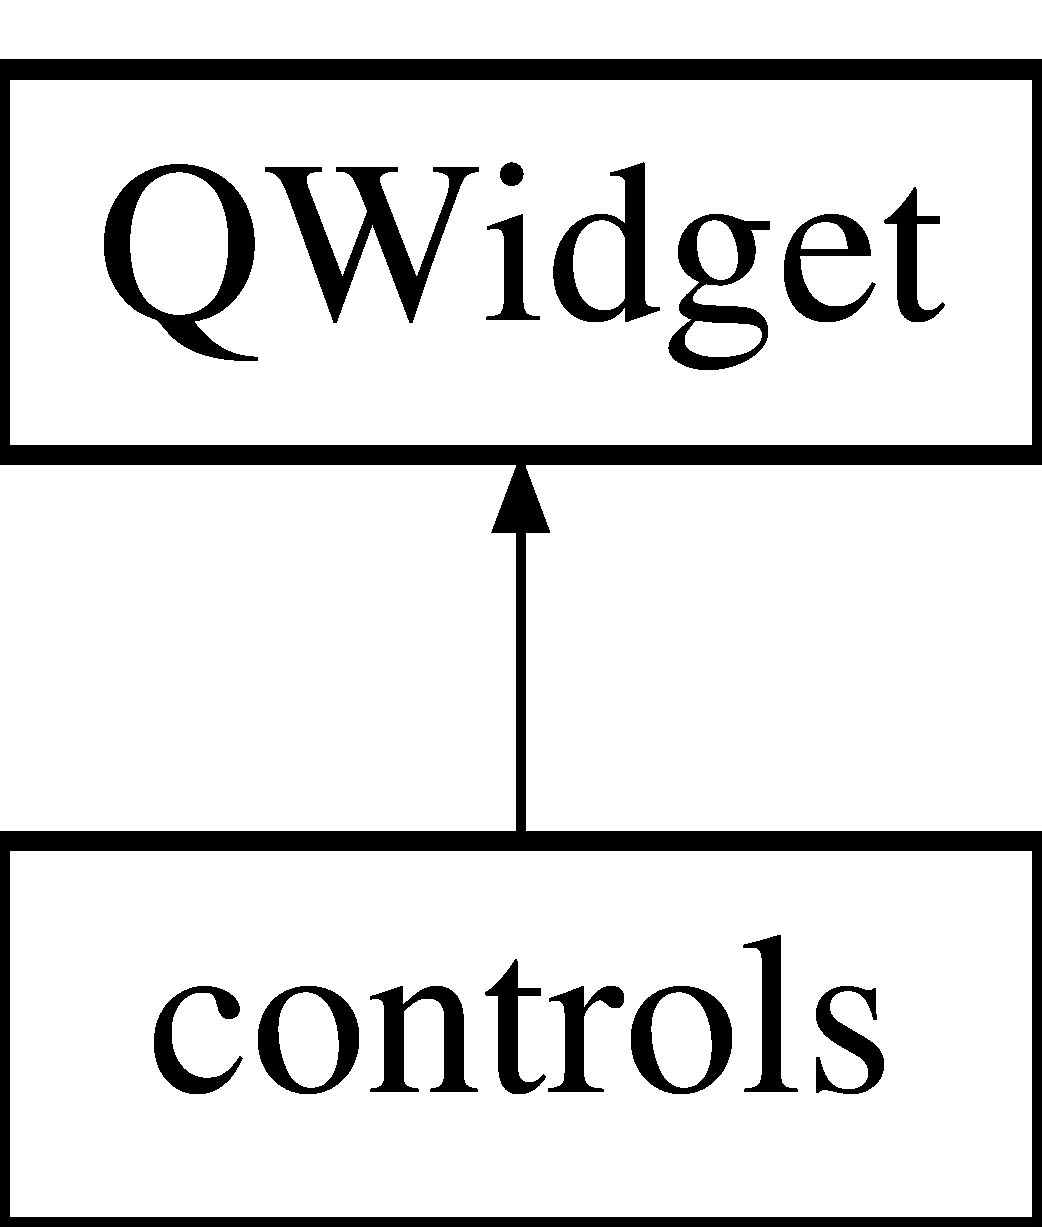
\includegraphics[height=2.000000cm]{classcontrols}
\end{center}
\end{figure}
\subsection*{Public Member Functions}
\begin{DoxyCompactItemize}
\item 
\hyperlink{classcontrols_a9a2803968e87a1d002044fbafcbad766}{controls} (Q\+Widget $\ast$parent=0)
\item 
\hyperlink{classcontrols_a69af1fa496cee3411b8d2f207f046786}{$\sim$controls} ()\hypertarget{classcontrols_a69af1fa496cee3411b8d2f207f046786}{}\label{classcontrols_a69af1fa496cee3411b8d2f207f046786}

\begin{DoxyCompactList}\small\item\em Deletes the UI. \end{DoxyCompactList}\item 
void \hyperlink{classcontrols_a61cf1ab9310885ff551b2393be8bab66}{paint\+Event} (Q\+Paint\+Event $\ast$)\hypertarget{classcontrols_a61cf1ab9310885ff551b2393be8bab66}{}\label{classcontrols_a61cf1ab9310885ff551b2393be8bab66}

\begin{DoxyCompactList}\small\item\em Fills the background with a black rectangle. \end{DoxyCompactList}\end{DoxyCompactItemize}


\subsection{Detailed Description}
This class handles the UI displaying the controls/instructions for the game. 

Definition at line 19 of file controls.\+h.



\subsection{Constructor \& Destructor Documentation}
\index{controls@{controls}!controls@{controls}}
\index{controls@{controls}!controls@{controls}}
\subsubsection[{\texorpdfstring{controls(\+Q\+Widget $\ast$parent=0)}{controls(QWidget *parent=0)}}]{\setlength{\rightskip}{0pt plus 5cm}controls\+::controls (
\begin{DoxyParamCaption}
\item[{Q\+Widget $\ast$}]{parent = {\ttfamily 0}}
\end{DoxyParamCaption}
)\hspace{0.3cm}{\ttfamily [explicit]}}\hypertarget{classcontrols_a9a2803968e87a1d002044fbafcbad766}{}\label{classcontrols_a9a2803968e87a1d002044fbafcbad766}
Constructs a controls object 
\begin{DoxyParams}{Parameters}
{\em parent} & is the parent Q\+Widget of this object \\
\hline
\end{DoxyParams}


Definition at line 8 of file controls.\+cpp.


\begin{DoxyCode}
8                                   : QWidget(parent), ui(\textcolor{keyword}{new} Ui::controls)
9 \{
10     \textcolor{comment}{// init ui form's components}
11     ui->setupUi(\textcolor{keyword}{this});
12     connect(ui->pushButton, SIGNAL(clicked(\textcolor{keywordtype}{bool})), parent, SLOT(game\_over()));
13 \}
\end{DoxyCode}


The documentation for this class was generated from the following files\+:\begin{DoxyCompactItemize}
\item 
\hyperlink{controls_8h}{controls.\+h}\item 
\hyperlink{controls_8cpp}{controls.\+cpp}\end{DoxyCompactItemize}

\hypertarget{classlevel1}{}\section{level1 Class Reference}
\label{classlevel1}\index{level1@{level1}}


This class handles the logic and display events for level 1.  




{\ttfamily \#include $<$level1.\+h$>$}

Inheritance diagram for level1\+:\begin{figure}[H]
\begin{center}
\leavevmode
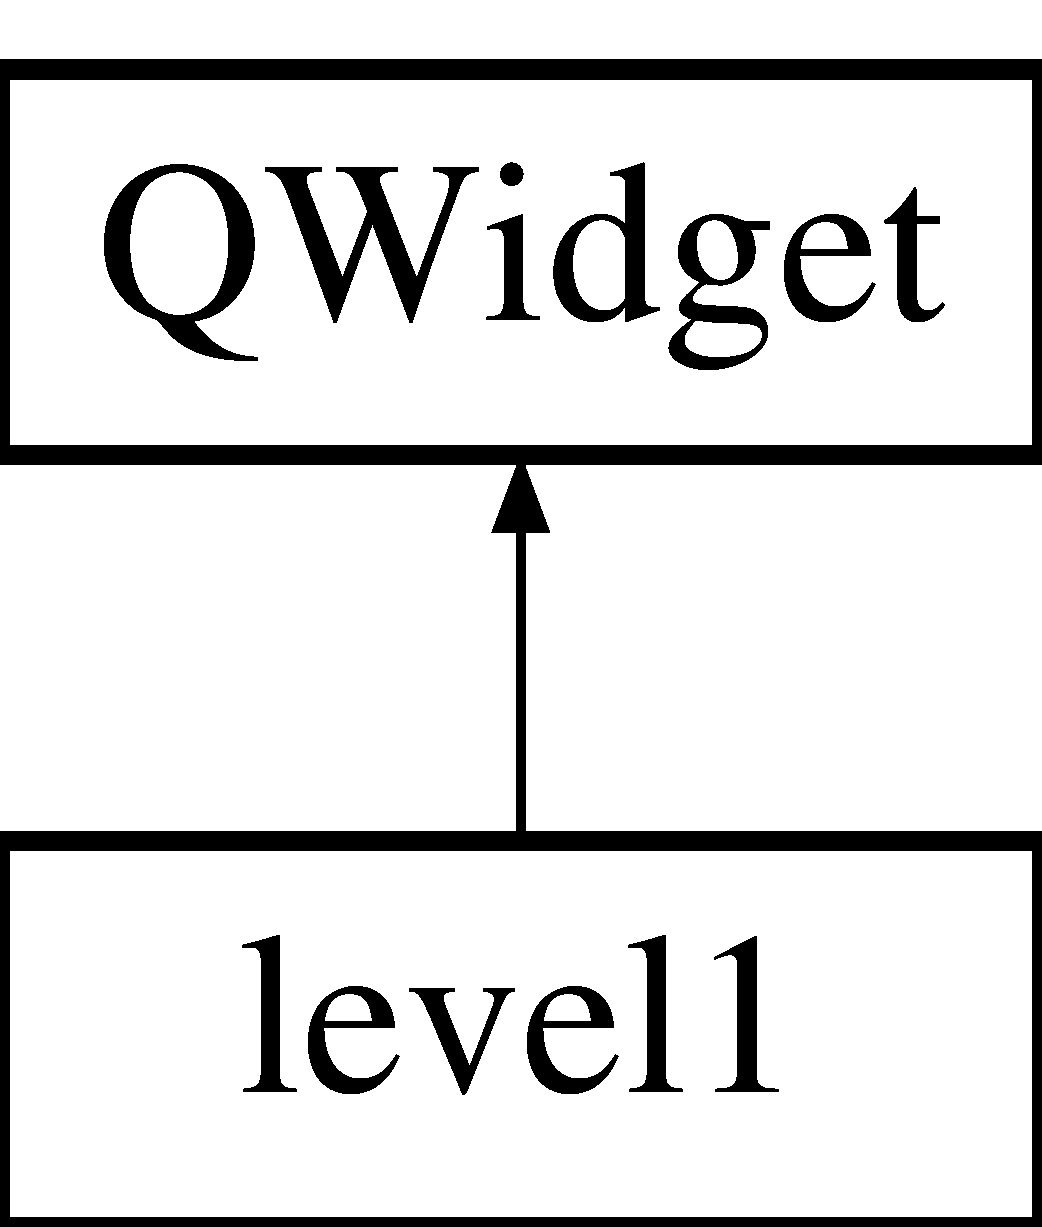
\includegraphics[height=2.000000cm]{classlevel1}
\end{center}
\end{figure}
\subsection*{Public Slots}
\begin{DoxyCompactItemize}
\item 
void \hyperlink{classlevel1_a431eac5dfc5286c4173d4ca18bef03ce}{update\+Frame} ()\hypertarget{classlevel1_a431eac5dfc5286c4173d4ca18bef03ce}{}\label{classlevel1_a431eac5dfc5286c4173d4ca18bef03ce}

\begin{DoxyCompactList}\small\item\em Scale the game to fit the current window dimensions. \end{DoxyCompactList}\item 
void \hyperlink{classlevel1_a20a0e78a0ea626784b2efd1addf82238}{animate\+Bullet} ()\hypertarget{classlevel1_a20a0e78a0ea626784b2efd1addf82238}{}\label{classlevel1_a20a0e78a0ea626784b2efd1addf82238}

\begin{DoxyCompactList}\small\item\em Handles the logic for animating the player\textquotesingle{}s bullet. \end{DoxyCompactList}\item 
void \hyperlink{classlevel1_a928d2376d442f285fa1e703a1a7f9104}{check\+Hitbox} ()\hypertarget{classlevel1_a928d2376d442f285fa1e703a1a7f9104}{}\label{classlevel1_a928d2376d442f285fa1e703a1a7f9104}

\begin{DoxyCompactList}\small\item\em Check player and enemy hitboxes for collisions. \end{DoxyCompactList}\item 
void \hyperlink{classlevel1_a76e8519c9cbae81ed94efac17e44565b}{animate\+Enemy} ()\hypertarget{classlevel1_a76e8519c9cbae81ed94efac17e44565b}{}\label{classlevel1_a76e8519c9cbae81ed94efac17e44565b}

\begin{DoxyCompactList}\small\item\em Handles the logic for moving the enemy and making the enemy attack. \end{DoxyCompactList}\item 
void \hyperlink{classlevel1_ace96df0a7bf2be129baa602a47ffc38d}{enemy\+Attack} ()\hypertarget{classlevel1_ace96df0a7bf2be129baa602a47ffc38d}{}\label{classlevel1_ace96df0a7bf2be129baa602a47ffc38d}

\begin{DoxyCompactList}\small\item\em Fires the enemy\textquotesingle{}s bullet. \end{DoxyCompactList}\end{DoxyCompactItemize}
\subsection*{Signals}
\begin{DoxyCompactItemize}
\item 
void \hyperlink{classlevel1_abc87b5eddf6272837ff28cb36d1df0ab}{game\+\_\+over} ()\hypertarget{classlevel1_abc87b5eddf6272837ff28cb36d1df0ab}{}\label{classlevel1_abc87b5eddf6272837ff28cb36d1df0ab}

\begin{DoxyCompactList}\small\item\em Signal called when the player has lost all of their lives. \end{DoxyCompactList}\item 
void \hyperlink{classlevel1_aaf762761c96d106b43fe0d331ecee122}{next\+\_\+level} ()\hypertarget{classlevel1_aaf762761c96d106b43fe0d331ecee122}{}\label{classlevel1_aaf762761c96d106b43fe0d331ecee122}

\begin{DoxyCompactList}\small\item\em Signal called when all enemies in the level have been defeated. \end{DoxyCompactList}\end{DoxyCompactItemize}
\subsection*{Public Member Functions}
\begin{DoxyCompactItemize}
\item 
\hyperlink{classlevel1_af9161b2438ae5d458fc142bd754a9000}{level1} (Q\+Widget $\ast$parent=0)
\item 
\hyperlink{classlevel1_a7346b26ad8d7c1e6101c55086ae1eed3}{$\sim$level1} ()\hypertarget{classlevel1_a7346b26ad8d7c1e6101c55086ae1eed3}{}\label{classlevel1_a7346b26ad8d7c1e6101c55086ae1eed3}

\begin{DoxyCompactList}\small\item\em Deletes the UI. \end{DoxyCompactList}\item 
void \hyperlink{classlevel1_ac47ea44681080d09e5d24bf14810f8ee}{paint\+Event} (Q\+Paint\+Event $\ast$)\hypertarget{classlevel1_ac47ea44681080d09e5d24bf14810f8ee}{}\label{classlevel1_ac47ea44681080d09e5d24bf14810f8ee}

\begin{DoxyCompactList}\small\item\em Draw all objects (player, enemies, bullets, etc.) onto the screen. \end{DoxyCompactList}\item 
void \hyperlink{classlevel1_a713dc5cfb6dd37be3979f48272680e2c}{key\+Press\+Event} (Q\+Key\+Event $\ast$e)
\item 
void \hyperlink{classlevel1_af7da421e6236bd4580d7ac6680e68be8}{show\+Event} (Q\+Show\+Event $\ast$e)
\end{DoxyCompactItemize}


\subsection{Detailed Description}
This class handles the logic and display events for level 1. 

Definition at line 30 of file level1.\+h.



\subsection{Constructor \& Destructor Documentation}
\index{level1@{level1}!level1@{level1}}
\index{level1@{level1}!level1@{level1}}
\subsubsection[{\texorpdfstring{level1(\+Q\+Widget $\ast$parent=0)}{level1(QWidget *parent=0)}}]{\setlength{\rightskip}{0pt plus 5cm}level1\+::level1 (
\begin{DoxyParamCaption}
\item[{Q\+Widget $\ast$}]{parent = {\ttfamily 0}}
\end{DoxyParamCaption}
)\hspace{0.3cm}{\ttfamily [explicit]}}\hypertarget{classlevel1_af9161b2438ae5d458fc142bd754a9000}{}\label{classlevel1_af9161b2438ae5d458fc142bd754a9000}
Create the level 
\begin{DoxyParams}{Parameters}
{\em parent} & is the parent Q\+Widget of this object \\
\hline
\end{DoxyParams}


Definition at line 9 of file level1.\+cpp.


\begin{DoxyCode}
9                               : QWidget(parent), ui(\textcolor{keyword}{new} Ui::level1)
10 \{
11     \textcolor{comment}{// init ui form's components}
12     ui->setupUi(\textcolor{keyword}{this});
13     \textcolor{comment}{// init pixmaps}
14     background = \textcolor{keyword}{new} QPixmap(\textcolor{stringliteral}{":/sprites/background.png"});
15     player = \textcolor{keyword}{new} QPixmap(\textcolor{stringliteral}{":/sprites/player.png"});
16     bullet = \textcolor{keyword}{new} QPixmap(\textcolor{stringliteral}{":/sprites/laser.png"});
17     enemy = \textcolor{keyword}{new} QPixmap(\textcolor{stringliteral}{":/sprites/enemy.png"});
18     enemyBullet = \textcolor{keyword}{new} QPixmap(\textcolor{stringliteral}{":/sprites/enemyLaser.png"});
19     \textcolor{comment}{// animate the bullet}
20     animateTimer = \textcolor{keyword}{new} QTimer();
21     connect(animateTimer, SIGNAL(timeout()), \textcolor{keyword}{this}, SLOT(\hyperlink{classlevel1_a20a0e78a0ea626784b2efd1addf82238}{animateBullet}()));
22     connect(animateTimer, SIGNAL(timeout()), \textcolor{keyword}{this}, SLOT(\hyperlink{classlevel1_a928d2376d442f285fa1e703a1a7f9104}{checkHitbox}()));
23     connect(animateTimer, SIGNAL(timeout()), \textcolor{keyword}{this}, SLOT(\hyperlink{classlevel1_a76e8519c9cbae81ed94efac17e44565b}{animateEnemy}()));
24     connect(animateTimer, SIGNAL(timeout()), \textcolor{keyword}{this}, SLOT(\hyperlink{classlevel1_a431eac5dfc5286c4173d4ca18bef03ce}{updateFrame}()));
25     animateTimer->start(40); \textcolor{comment}{// timer times out every 40 ms}
26     \textcolor{comment}{// enemy attacks every 5 seconds}
27     attackTimer = \textcolor{keyword}{new} QTimer();
28     connect(attackTimer, SIGNAL(timeout()), \textcolor{keyword}{this}, SLOT(\hyperlink{classlevel1_ace96df0a7bf2be129baa602a47ffc38d}{enemyAttack}()));
29     attackTimer->start(3000); \textcolor{comment}{// timer times out every 5 secs}
30     \textcolor{comment}{// init scoreboard stats}
31     lives = 3;
32     score = 0;
33     \textcolor{comment}{// game over and next level events}
34     connect(\textcolor{keyword}{this}, SIGNAL(\hyperlink{classlevel1_abc87b5eddf6272837ff28cb36d1df0ab}{game\_over}()), parent, SLOT(\hyperlink{classlevel1_abc87b5eddf6272837ff28cb36d1df0ab}{game\_over}()));
35     connect(\textcolor{keyword}{this}, SIGNAL(\hyperlink{classlevel1_aaf762761c96d106b43fe0d331ecee122}{next\_level}()), parent, SLOT(start\_level2()));
36     \textcolor{comment}{// sounds}
37     bulletSound = \textcolor{keyword}{new} QMediaPlayer();
38     bulletSound->setMedia(QUrl(\textcolor{stringliteral}{"qrc:/sounds/laser.mp3"}));
39     enemySound = \textcolor{keyword}{new} QMediaPlayer();
40     enemySound->setMedia(QUrl(\textcolor{stringliteral}{"qrc:/sounds/enemylaser.wav"}));
41     deathSound = \textcolor{keyword}{new} QMediaPlayer();
42     deathSound->setMedia((QUrl(\textcolor{stringliteral}{"qrc:/sounds/death.mp3"})));
43 \}
\end{DoxyCode}


\subsection{Member Function Documentation}
\index{level1@{level1}!key\+Press\+Event@{key\+Press\+Event}}
\index{key\+Press\+Event@{key\+Press\+Event}!level1@{level1}}
\subsubsection[{\texorpdfstring{key\+Press\+Event(\+Q\+Key\+Event $\ast$e)}{keyPressEvent(QKeyEvent *e)}}]{\setlength{\rightskip}{0pt plus 5cm}void level1\+::key\+Press\+Event (
\begin{DoxyParamCaption}
\item[{Q\+Key\+Event $\ast$}]{e}
\end{DoxyParamCaption}
)}\hypertarget{classlevel1_a713dc5cfb6dd37be3979f48272680e2c}{}\label{classlevel1_a713dc5cfb6dd37be3979f48272680e2c}
Handle keyboard input. Left and right keys move the player, space shoots a bullet. 
\begin{DoxyParams}{Parameters}
{\em e} & is the event corresponding with each keypress \\
\hline
\end{DoxyParams}


Definition at line 71 of file level1.\+cpp.


\begin{DoxyCode}
72 \{
73     \textcolor{comment}{// player cannot go off of the screen}
74     \textcolor{keywordflow}{if} (e->key() == Qt::Key\_Left) \{
75         \textcolor{keywordflow}{if} (playerLoc->x() > 0)
76             playerLoc->setX(playerLoc->x()-playerSpeed);
77     \}
78     \textcolor{keywordflow}{else} \textcolor{keywordflow}{if} (e->key() == Qt::Key\_Right) \{
79         \textcolor{keywordflow}{if} (playerLoc->x() + playerSize->width() < this->width())
80             playerLoc->setX(playerLoc->x()+playerSpeed);
81     \}
82     \textcolor{comment}{// player can only fire one bullet at a time}
83     \textcolor{keywordflow}{else} \textcolor{keywordflow}{if} (e->key() == Qt::Key\_Space) \{
84         \textcolor{keywordflow}{if} (canFire) \{
85             bulletLoc = \textcolor{keyword}{new} QPoint(playerLoc->x()+(bulletSize->width()/2), playerLoc->y() - bulletSize->
      height()/2);
86             \textcolor{keywordflow}{if} (bulletSound->state() == QMediaPlayer::PlayingState)
87                 bulletSound->setPosition(0);
88             bulletSound->play();
89             canFire = \textcolor{keyword}{false};
90         \}
91     \}
92     \textcolor{comment}{// repaint the scene}
93     this->update();
94 \}
\end{DoxyCode}
\index{level1@{level1}!show\+Event@{show\+Event}}
\index{show\+Event@{show\+Event}!level1@{level1}}
\subsubsection[{\texorpdfstring{show\+Event(\+Q\+Show\+Event $\ast$e)}{showEvent(QShowEvent *e)}}]{\setlength{\rightskip}{0pt plus 5cm}void level1\+::show\+Event (
\begin{DoxyParamCaption}
\item[{Q\+Show\+Event $\ast$}]{e}
\end{DoxyParamCaption}
)}\hypertarget{classlevel1_af7da421e6236bd4580d7ac6680e68be8}{}\label{classlevel1_af7da421e6236bd4580d7ac6680e68be8}
Initialize specific class variables when the Q\+Widget is shown 
\begin{DoxyParams}{Parameters}
{\em e} & is the event object created when the Q\+Widget is first displayed on screen \\
\hline
\end{DoxyParams}


Definition at line 96 of file level1.\+cpp.


\begin{DoxyCode}
97 \{
98     \textcolor{comment}{// show the widget and allow it to take keyboard input}
99     this->activateWindow();
100     this->setFocus();
101     QWidget::showEvent(e);
102     \textcolor{comment}{// init player variables}
103     playerAlive = \textcolor{keyword}{true};
104     playerSpeed = this->width()/50;
105     playerSize = \textcolor{keyword}{new} QSize(this->width()/18, this->width()/10);
106     \textcolor{comment}{// player starts in the middle-bottom of the screen}
107     playerLoc = \textcolor{keyword}{new} QPoint((this->width()/2)-playerSize->width(), this->height() - playerSize->height());
108     canFire = \textcolor{keyword}{true}; \textcolor{comment}{// player is able to shoot}
109     \textcolor{comment}{// init bullet size and speed}
110     bulletSize = \textcolor{keyword}{new} QSize(playerSize->width()/2, playerSize->height()/2);
111     bulletSpeed = this->height()/50;
112     \textcolor{comment}{// init enemy variables}
113     enemyAlive = \textcolor{keyword}{true};
114     left = \textcolor{keyword}{false};
115     enemySpeed = this->width()/200;
116     enemySize = \textcolor{keyword}{new} QSize(this->width()/18, this->width()/10);
117     \textcolor{comment}{// enemy starts in the middle-top of the screen}
118     enemyLoc = \textcolor{keyword}{new} QPoint((this->width()/2)-enemySize->width(), 0 + enemySize->height()/3);
119     enemyCanFire = \textcolor{keyword}{true};
120 \}
\end{DoxyCode}


The documentation for this class was generated from the following files\+:\begin{DoxyCompactItemize}
\item 
\hyperlink{level1_8h}{level1.\+h}\item 
\hyperlink{level1_8cpp}{level1.\+cpp}\end{DoxyCompactItemize}

\hypertarget{classlevel2}{}\section{level2 Class Reference}
\label{classlevel2}\index{level2@{level2}}


This class handles the logic and display events for level 2.  




{\ttfamily \#include $<$level2.\+h$>$}

Inheritance diagram for level2\+:\begin{figure}[H]
\begin{center}
\leavevmode
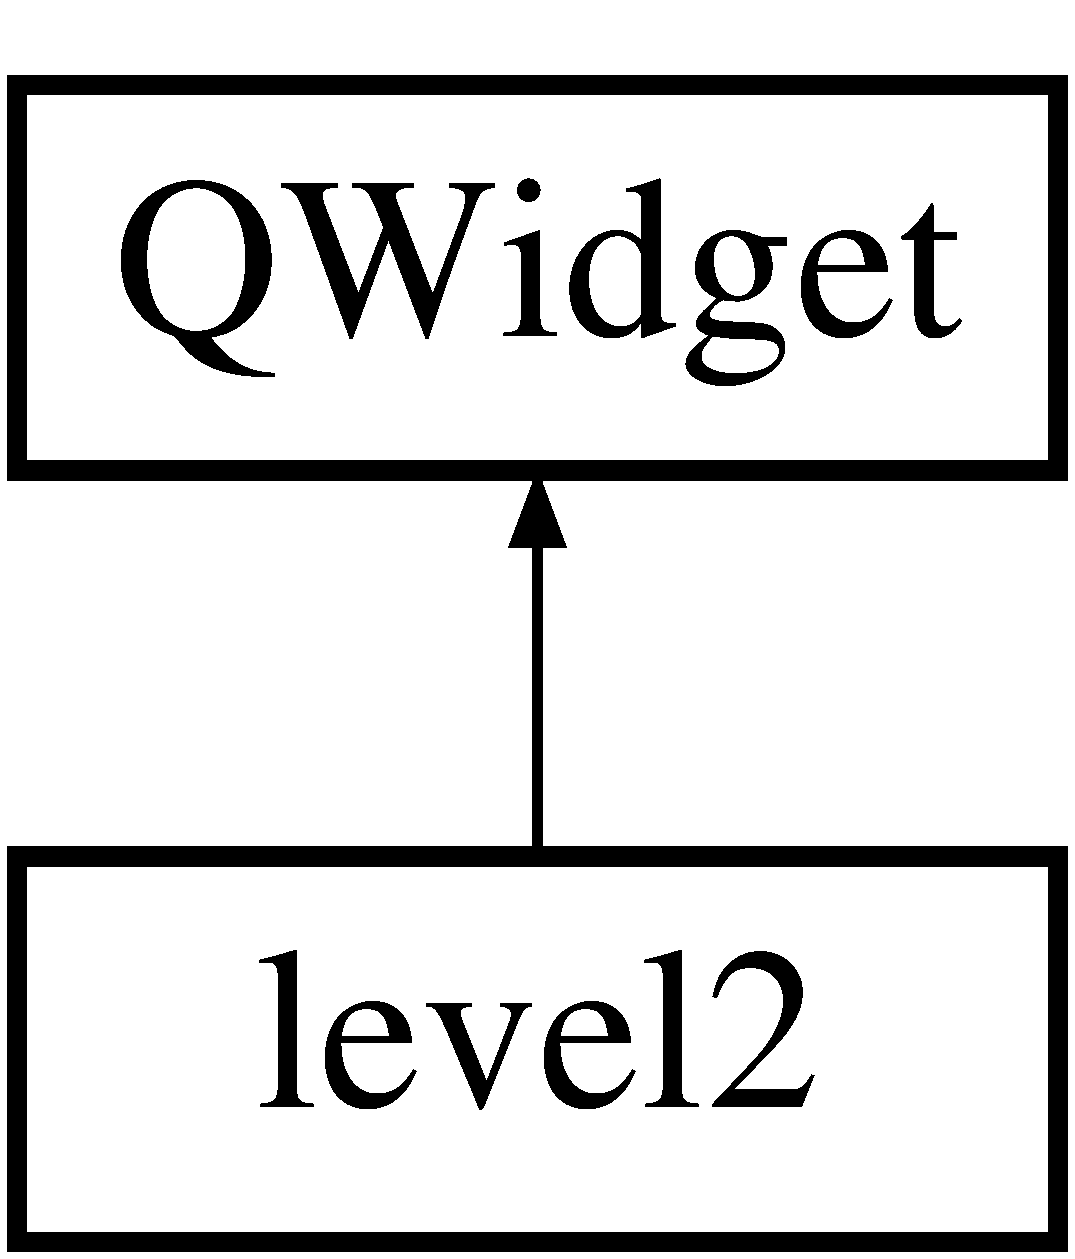
\includegraphics[height=2.000000cm]{classlevel2}
\end{center}
\end{figure}
\subsection*{Public Slots}
\begin{DoxyCompactItemize}
\item 
void \hyperlink{classlevel2_a4a0d1f53743f3e6d703dc964889b9fb1}{update\+Frame} ()\hypertarget{classlevel2_a4a0d1f53743f3e6d703dc964889b9fb1}{}\label{classlevel2_a4a0d1f53743f3e6d703dc964889b9fb1}

\begin{DoxyCompactList}\small\item\em Scale the game to fit the current window dimensions. \end{DoxyCompactList}\item 
void \hyperlink{classlevel2_ae16aee7a8edd8fe1c52ff9e9a7b88017}{animate\+Bullet} ()\hypertarget{classlevel2_ae16aee7a8edd8fe1c52ff9e9a7b88017}{}\label{classlevel2_ae16aee7a8edd8fe1c52ff9e9a7b88017}

\begin{DoxyCompactList}\small\item\em Handles the logic for animating the player\textquotesingle{}s bullet. \end{DoxyCompactList}\item 
void \hyperlink{classlevel2_a636ce0136ade6b52f93d6addcb5a4274}{check\+Hitbox} ()\hypertarget{classlevel2_a636ce0136ade6b52f93d6addcb5a4274}{}\label{classlevel2_a636ce0136ade6b52f93d6addcb5a4274}

\begin{DoxyCompactList}\small\item\em Check player and enemy hitboxes for collisions. \end{DoxyCompactList}\item 
void \hyperlink{classlevel2_a8ac4c147da9cf53e5da58f265b8ae27c}{animate\+Enemy} ()\hypertarget{classlevel2_a8ac4c147da9cf53e5da58f265b8ae27c}{}\label{classlevel2_a8ac4c147da9cf53e5da58f265b8ae27c}

\begin{DoxyCompactList}\small\item\em Handles the logic for moving the enemy and making the enemy attack. \end{DoxyCompactList}\item 
void \hyperlink{classlevel2_a751ea7e83ef9372f79e0fedc77ce5088}{enemy\+Attack} ()\hypertarget{classlevel2_a751ea7e83ef9372f79e0fedc77ce5088}{}\label{classlevel2_a751ea7e83ef9372f79e0fedc77ce5088}

\begin{DoxyCompactList}\small\item\em Fires the enemy\textquotesingle{}s bullet. \end{DoxyCompactList}\end{DoxyCompactItemize}
\subsection*{Signals}
\begin{DoxyCompactItemize}
\item 
void \hyperlink{classlevel2_a688ffd62097bfe0e62e16c34f4b0c0fb}{game\+\_\+over} ()\hypertarget{classlevel2_a688ffd62097bfe0e62e16c34f4b0c0fb}{}\label{classlevel2_a688ffd62097bfe0e62e16c34f4b0c0fb}

\begin{DoxyCompactList}\small\item\em Signal called when the player has lost all of their lives. \end{DoxyCompactList}\item 
void \hyperlink{classlevel2_ab9639c124108ea3170de5051f9016151}{next\+\_\+level} ()\hypertarget{classlevel2_ab9639c124108ea3170de5051f9016151}{}\label{classlevel2_ab9639c124108ea3170de5051f9016151}

\begin{DoxyCompactList}\small\item\em Signal called when all enemies in the level have been defeated. \end{DoxyCompactList}\end{DoxyCompactItemize}
\subsection*{Public Member Functions}
\begin{DoxyCompactItemize}
\item 
\hyperlink{classlevel2_a60e8d70343c4d2aee2eb4fff186d9052}{level2} (Q\+Widget $\ast$parent=0)
\item 
\hyperlink{classlevel2_a1088443fbe07a629a2f5fb8874dce992}{$\sim$level2} ()\hypertarget{classlevel2_a1088443fbe07a629a2f5fb8874dce992}{}\label{classlevel2_a1088443fbe07a629a2f5fb8874dce992}

\begin{DoxyCompactList}\small\item\em Deletes the UI. \end{DoxyCompactList}\item 
void \hyperlink{classlevel2_ae9d1427d9d57a2c4eee057c55106438a}{paint\+Event} (Q\+Paint\+Event $\ast$)\hypertarget{classlevel2_ae9d1427d9d57a2c4eee057c55106438a}{}\label{classlevel2_ae9d1427d9d57a2c4eee057c55106438a}

\begin{DoxyCompactList}\small\item\em Draw all objects (player, enemies, bullets, etc.) onto the screen. \end{DoxyCompactList}\item 
void \hyperlink{classlevel2_aaf795c710bf3fe689cc1b8a8aafc07a5}{key\+Press\+Event} (Q\+Key\+Event $\ast$e)
\item 
void \hyperlink{classlevel2_abbc04545229e166ac0195f37cabb3908}{show\+Event} (Q\+Show\+Event $\ast$e)
\item 
void \hyperlink{classlevel2_a18024c7ee849253b6c395a8d94c5bdc4}{move\+Enemy} (Q\+Point $\ast$enemy)
\item 
bool \hyperlink{classlevel2_af18eec7d678db9d70448eb9ad1e7292f}{enemy\+Hit} (Q\+Point $\ast$enemy)
\end{DoxyCompactItemize}


\subsection{Detailed Description}
This class handles the logic and display events for level 2. 

Definition at line 33 of file level2.\+h.



\subsection{Constructor \& Destructor Documentation}
\index{level2@{level2}!level2@{level2}}
\index{level2@{level2}!level2@{level2}}
\subsubsection[{\texorpdfstring{level2(\+Q\+Widget $\ast$parent=0)}{level2(QWidget *parent=0)}}]{\setlength{\rightskip}{0pt plus 5cm}level2\+::level2 (
\begin{DoxyParamCaption}
\item[{Q\+Widget $\ast$}]{parent = {\ttfamily 0}}
\end{DoxyParamCaption}
)\hspace{0.3cm}{\ttfamily [explicit]}}\hypertarget{classlevel2_a60e8d70343c4d2aee2eb4fff186d9052}{}\label{classlevel2_a60e8d70343c4d2aee2eb4fff186d9052}
Create the level 
\begin{DoxyParams}{Parameters}
{\em parent} & is the parent Q\+Widget of this object \\
\hline
\end{DoxyParams}


Definition at line 9 of file level2.\+cpp.


\begin{DoxyCode}
9                               : QWidget(parent), ui(\textcolor{keyword}{new} Ui::level2)
10 \{
11     \textcolor{comment}{// init ui form's components}
12     ui->setupUi(\textcolor{keyword}{this});
13     \textcolor{comment}{// init pixmaps}
14     background = \textcolor{keyword}{new} QPixmap(\textcolor{stringliteral}{":/sprites/background.png"});
15     player = \textcolor{keyword}{new} QPixmap(\textcolor{stringliteral}{":/sprites/player.png"});
16     bullet = \textcolor{keyword}{new} QPixmap(\textcolor{stringliteral}{":/sprites/laser.png"});
17     enemy = \textcolor{keyword}{new} QPixmap(\textcolor{stringliteral}{":/sprites/enemy2.png"});
18     enemyBullet = \textcolor{keyword}{new} QPixmap(\textcolor{stringliteral}{":/sprites/bossAttack.png"});
19     \textcolor{comment}{// animate the bullet}
20     animateTimer = \textcolor{keyword}{new} QTimer();
21     connect(animateTimer, SIGNAL(timeout()), \textcolor{keyword}{this}, SLOT(\hyperlink{classlevel2_ae16aee7a8edd8fe1c52ff9e9a7b88017}{animateBullet}()));
22     connect(animateTimer, SIGNAL(timeout()), \textcolor{keyword}{this}, SLOT(\hyperlink{classlevel2_a636ce0136ade6b52f93d6addcb5a4274}{checkHitbox}()));
23     connect(animateTimer, SIGNAL(timeout()), \textcolor{keyword}{this}, SLOT(\hyperlink{classlevel2_a8ac4c147da9cf53e5da58f265b8ae27c}{animateEnemy}()));
24     connect(animateTimer, SIGNAL(timeout()), \textcolor{keyword}{this}, SLOT(\hyperlink{classlevel2_a4a0d1f53743f3e6d703dc964889b9fb1}{updateFrame}()));
25     animateTimer->start(40); \textcolor{comment}{// timer times out every 40 ms}
26     \textcolor{comment}{// enemy attacks every 5 seconds}
27     attackTimer = \textcolor{keyword}{new} QTimer();
28     connect(attackTimer, SIGNAL(timeout()), \textcolor{keyword}{this}, SLOT(\hyperlink{classlevel2_a751ea7e83ef9372f79e0fedc77ce5088}{enemyAttack}()));
29     attackTimer->start(3000); \textcolor{comment}{// timer times out every 5 secs}
30     \textcolor{comment}{// init scoreboard stats}
31     lives = 3;
32     score = 0;
33     \textcolor{comment}{// game over and next level events}
34     connect(\textcolor{keyword}{this}, SIGNAL(\hyperlink{classlevel2_a688ffd62097bfe0e62e16c34f4b0c0fb}{game\_over}()), parent, SLOT(\hyperlink{classlevel2_a688ffd62097bfe0e62e16c34f4b0c0fb}{game\_over}()));
35     connect(\textcolor{keyword}{this}, SIGNAL(\hyperlink{classlevel2_ab9639c124108ea3170de5051f9016151}{next\_level}()), parent, SLOT(start\_level3()));
36     \textcolor{comment}{// seed rng}
37     \textcolor{keywordtype}{unsigned} \textcolor{keywordtype}{int} seed = std::chrono::system\_clock().now().time\_since\_epoch().count();
38     generator = std::default\_random\_engine(seed);
39     unif = std::uniform\_int\_distribution<int>(1,4);
40     \textcolor{comment}{// sounds}
41     bulletSound = \textcolor{keyword}{new} QMediaPlayer();
42     bulletSound->setMedia(QUrl(\textcolor{stringliteral}{"qrc:/sounds/laser.mp3"}));
43     enemySound = \textcolor{keyword}{new} QMediaPlayer();
44     enemySound->setMedia(QUrl(\textcolor{stringliteral}{"qrc:/sounds/enemylaser.wav"}));
45     deathSound = \textcolor{keyword}{new} QMediaPlayer();
46     deathSound->setMedia((QUrl(\textcolor{stringliteral}{"qrc:/sounds/death.mp3"})));
47 \}
\end{DoxyCode}


\subsection{Member Function Documentation}
\index{level2@{level2}!enemy\+Hit@{enemy\+Hit}}
\index{enemy\+Hit@{enemy\+Hit}!level2@{level2}}
\subsubsection[{\texorpdfstring{enemy\+Hit(\+Q\+Point $\ast$enemy)}{enemyHit(QPoint *enemy)}}]{\setlength{\rightskip}{0pt plus 5cm}bool level2\+::enemy\+Hit (
\begin{DoxyParamCaption}
\item[{Q\+Point $\ast$}]{enemy}
\end{DoxyParamCaption}
)}\hypertarget{classlevel2_af18eec7d678db9d70448eb9ad1e7292f}{}\label{classlevel2_af18eec7d678db9d70448eb9ad1e7292f}
Checks whether an enemy was hit by the player\textquotesingle{}s bullet 
\begin{DoxyParams}{Parameters}
{\em enemy} & checks the given enemy for collisions with the player\textquotesingle{}s bullet \\
\hline
\end{DoxyParams}


Definition at line 159 of file level2.\+cpp.


\begin{DoxyCode}
160 \{
161     \textcolor{keywordflow}{if} (bulletLoc->y() < enemy->y() + enemySize->height()/2 &&
162             bulletLoc->x() + bulletSize->width() > enemy->x() &&
163             bulletLoc->x() < enemy->x() + enemySize->width()) \{
164         \textcolor{keywordflow}{return} \textcolor{keyword}{true};
165     \}
166     \textcolor{keywordflow}{return} \textcolor{keyword}{false};
167 \}
\end{DoxyCode}
\index{level2@{level2}!key\+Press\+Event@{key\+Press\+Event}}
\index{key\+Press\+Event@{key\+Press\+Event}!level2@{level2}}
\subsubsection[{\texorpdfstring{key\+Press\+Event(\+Q\+Key\+Event $\ast$e)}{keyPressEvent(QKeyEvent *e)}}]{\setlength{\rightskip}{0pt plus 5cm}void level2\+::key\+Press\+Event (
\begin{DoxyParamCaption}
\item[{Q\+Key\+Event $\ast$}]{e}
\end{DoxyParamCaption}
)}\hypertarget{classlevel2_aaf795c710bf3fe689cc1b8a8aafc07a5}{}\label{classlevel2_aaf795c710bf3fe689cc1b8a8aafc07a5}
Handle keyboard input. Left and right keys move the player, space shoots a bullet. 
\begin{DoxyParams}{Parameters}
{\em e} & is the event corresponding with each keypress \\
\hline
\end{DoxyParams}


Definition at line 81 of file level2.\+cpp.


\begin{DoxyCode}
82 \{
83     \textcolor{comment}{// player cannot go off of the screen}
84     \textcolor{keywordflow}{if} (e->key() == Qt::Key\_Left) \{
85         \textcolor{keywordflow}{if} (playerLoc->x() > 0)
86             playerLoc->setX(playerLoc->x()-playerSpeed);
87     \}
88     \textcolor{keywordflow}{else} \textcolor{keywordflow}{if} (e->key() == Qt::Key\_Right) \{
89         \textcolor{keywordflow}{if} (playerLoc->x() + playerSize->width() < this->width())
90             playerLoc->setX(playerLoc->x()+playerSpeed);
91     \}
92     \textcolor{comment}{// player can only fire one bullet at a time}
93     \textcolor{keywordflow}{else} \textcolor{keywordflow}{if} (e->key() == Qt::Key\_Space) \{
94         \textcolor{keywordflow}{if} (canFire) \{
95             bulletLoc = \textcolor{keyword}{new} QPoint(playerLoc->x()+(bulletSize->width()/2), playerLoc->y() - bulletSize->
      height()/2);
96             \textcolor{keywordflow}{if} (bulletSound->state() == QMediaPlayer::PlayingState)
97                 bulletSound->setPosition(0);
98             bulletSound->play();
99             canFire = \textcolor{keyword}{false};
100         \}
101     \}
102     \textcolor{comment}{// repaint the scene}
103     this->update();
104 \}
\end{DoxyCode}
\index{level2@{level2}!move\+Enemy@{move\+Enemy}}
\index{move\+Enemy@{move\+Enemy}!level2@{level2}}
\subsubsection[{\texorpdfstring{move\+Enemy(\+Q\+Point $\ast$enemy)}{moveEnemy(QPoint *enemy)}}]{\setlength{\rightskip}{0pt plus 5cm}void level2\+::move\+Enemy (
\begin{DoxyParamCaption}
\item[{Q\+Point $\ast$}]{enemy}
\end{DoxyParamCaption}
)}\hypertarget{classlevel2_a18024c7ee849253b6c395a8d94c5bdc4}{}\label{classlevel2_a18024c7ee849253b6c395a8d94c5bdc4}
Moves the enemy back and forth across the screen. 
\begin{DoxyParams}{Parameters}
{\em enemy} & is the enemy that we want to move around on the screen \\
\hline
\end{DoxyParams}


Definition at line 142 of file level2.\+cpp.


\begin{DoxyCode}
143 \{
144     \textcolor{comment}{// enemy moves left until it hits the right part of the screen}
145     \textcolor{keywordflow}{if} (left && enemy->x() > 0) \{
146         enemy->setX(enemy->x() - enemySpeed);
147     \}
148     \textcolor{comment}{// enemy moves right until it hits the left part of the screen}
149     \textcolor{keywordflow}{else} \textcolor{keywordflow}{if} (!left && enemy->x() + enemySize->width() < this->width()) \{
150         enemy->setX(enemy->x() + enemySpeed);
151     \}
152     \textcolor{comment}{// flip direction}
153     \textcolor{keywordflow}{else} \{
154         left = !left;
155     \}
156     update();
157 \}
\end{DoxyCode}
\index{level2@{level2}!show\+Event@{show\+Event}}
\index{show\+Event@{show\+Event}!level2@{level2}}
\subsubsection[{\texorpdfstring{show\+Event(\+Q\+Show\+Event $\ast$e)}{showEvent(QShowEvent *e)}}]{\setlength{\rightskip}{0pt plus 5cm}void level2\+::show\+Event (
\begin{DoxyParamCaption}
\item[{Q\+Show\+Event $\ast$}]{e}
\end{DoxyParamCaption}
)}\hypertarget{classlevel2_abbc04545229e166ac0195f37cabb3908}{}\label{classlevel2_abbc04545229e166ac0195f37cabb3908}
Initialize specific class variables when the Q\+Widget is shown 
\begin{DoxyParams}{Parameters}
{\em e} & is the event object created when the Q\+Widget is first displayed on screen \\
\hline
\end{DoxyParams}


Definition at line 106 of file level2.\+cpp.


\begin{DoxyCode}
107 \{
108     \textcolor{comment}{// show the widget and allow it to take keyboard input}
109     this->activateWindow();
110     this->setFocus();
111     QWidget::showEvent(e);
112     \textcolor{comment}{// init player variables}
113     playerAlive = \textcolor{keyword}{true};
114     playerSpeed = this->width()/50;
115     playerSize = \textcolor{keyword}{new} QSize(this->width()/18, this->width()/10);
116     \textcolor{comment}{// player starts in the middle-bottom of the screen}
117     playerLoc = \textcolor{keyword}{new} QPoint((this->width()/2)-playerSize->width(), this->height() - playerSize->height());
118     canFire = \textcolor{keyword}{true}; \textcolor{comment}{// player is able to shoot}
119     \textcolor{comment}{// init enemy variables}
120     enemyAlive = \textcolor{keyword}{true};
121     left = \textcolor{keyword}{false};
122     enemySpeed = this->width()/200;
123     enemySize = \textcolor{keyword}{new} QSize(this->width()/10, this->width()/10);
124     \textcolor{comment}{// enemy starts in the middle-top of the screen}
125     enemyLoc = \textcolor{keyword}{new} QPoint((this->width()/2)-enemySize->width(), 0 + enemySize->height()/3);
126     enemyCanFire = \textcolor{keyword}{true};
127     \textcolor{comment}{// enemy2 variables}
128     enemy2Loc = \textcolor{keyword}{new} QPoint((this->width()/2)-2*enemySize->width(), 0 + enemySize->height()/3);
129     enemy2Alive = \textcolor{keyword}{true};
130     \textcolor{comment}{// enemy3 variables}
131     enemy3Loc = \textcolor{keyword}{new} QPoint((this->width()/2)-3*enemySize->width(), 0 + enemySize->height()/3);
132     enemy3Alive = \textcolor{keyword}{true};
133     \textcolor{comment}{// enemy4 variables}
134     enemy4Loc = \textcolor{keyword}{new} QPoint((this->width()/2)-4*enemySize->width(), 0 + enemySize->height()/3);
135     enemy4Alive = \textcolor{keyword}{true};
136     \textcolor{comment}{// init bullet size and speed}
137     bulletSize = \textcolor{keyword}{new} QSize(playerSize->width()/2, playerSize->height()/2);
138     enemyBulletSize = \textcolor{keyword}{new} QSize(enemySize->width()/4, enemySize->width()/2);
139     bulletSpeed = this->height()/50;
140 \}
\end{DoxyCode}


The documentation for this class was generated from the following files\+:\begin{DoxyCompactItemize}
\item 
\hyperlink{level2_8h}{level2.\+h}\item 
\hyperlink{level2_8cpp}{level2.\+cpp}\end{DoxyCompactItemize}

\hypertarget{classlevel3}{}\section{level3 Class Reference}
\label{classlevel3}\index{level3@{level3}}


This class handles the logic and display events for level 3.  




{\ttfamily \#include $<$level3.\+h$>$}

Inheritance diagram for level3\+:\begin{figure}[H]
\begin{center}
\leavevmode
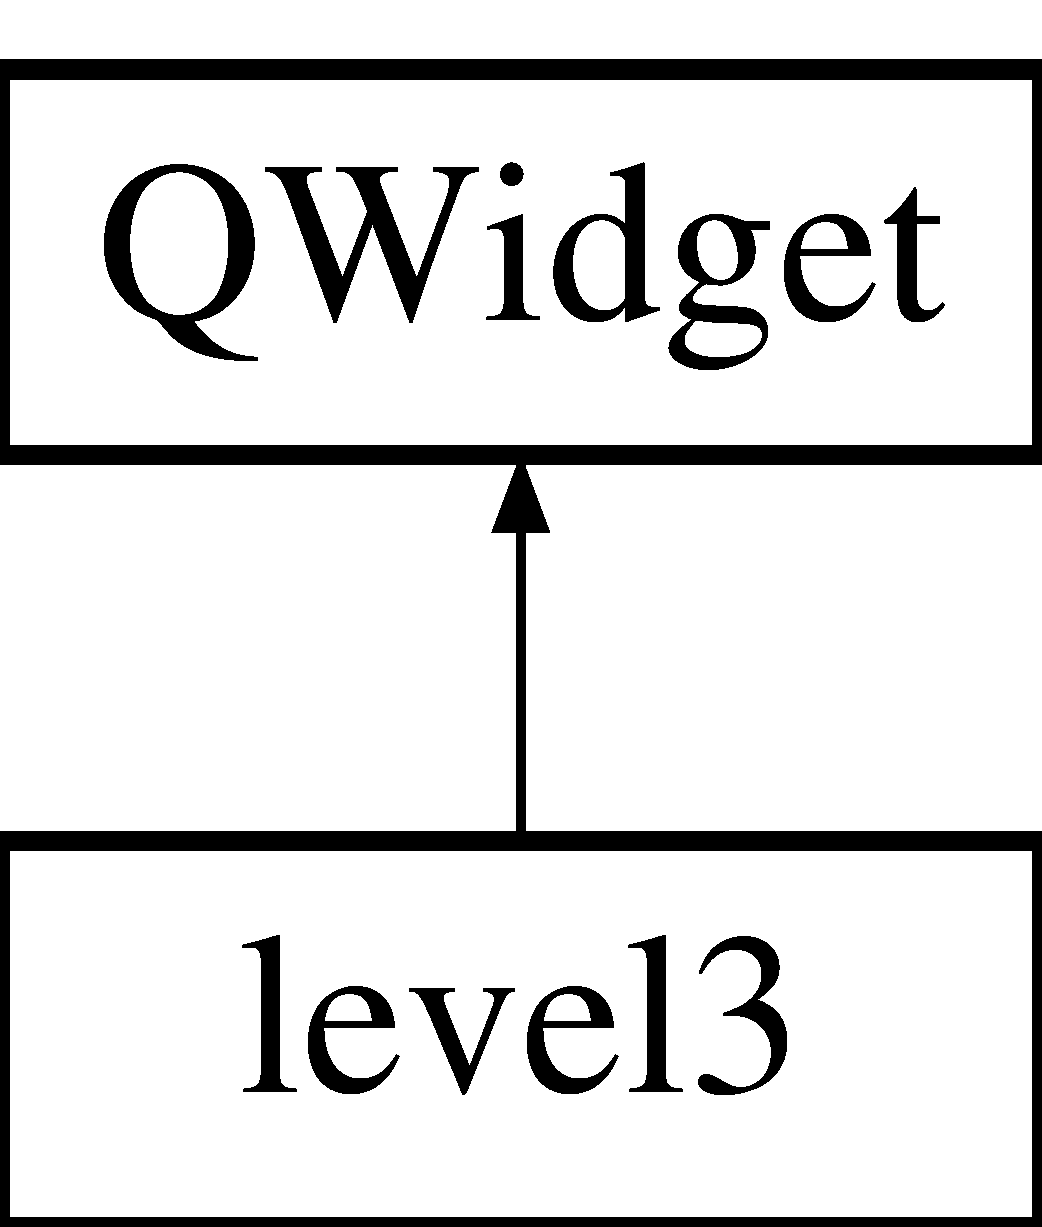
\includegraphics[height=2.000000cm]{classlevel3}
\end{center}
\end{figure}
\subsection*{Public Slots}
\begin{DoxyCompactItemize}
\item 
void \hyperlink{classlevel3_a1829c75ea73f9cd85d508609dc07e6d6}{update\+Frame} ()\hypertarget{classlevel3_a1829c75ea73f9cd85d508609dc07e6d6}{}\label{classlevel3_a1829c75ea73f9cd85d508609dc07e6d6}

\begin{DoxyCompactList}\small\item\em Scale the game to fit the current window dimensions. \end{DoxyCompactList}\item 
void \hyperlink{classlevel3_a83c0241cb42c34c707758adff87a4b49}{animate\+Bullet} ()\hypertarget{classlevel3_a83c0241cb42c34c707758adff87a4b49}{}\label{classlevel3_a83c0241cb42c34c707758adff87a4b49}

\begin{DoxyCompactList}\small\item\em Handles the logic for animating the player\textquotesingle{}s bullet. \end{DoxyCompactList}\item 
void \hyperlink{classlevel3_a8b8f7f12a1fcafc61cb61d73c82ff900}{check\+Hitbox} ()\hypertarget{classlevel3_a8b8f7f12a1fcafc61cb61d73c82ff900}{}\label{classlevel3_a8b8f7f12a1fcafc61cb61d73c82ff900}

\begin{DoxyCompactList}\small\item\em Check player and enemy hitboxes for collisions. \end{DoxyCompactList}\item 
void \hyperlink{classlevel3_ab413227813899b1d0aefa085ede06df0}{animate\+Enemy} ()\hypertarget{classlevel3_ab413227813899b1d0aefa085ede06df0}{}\label{classlevel3_ab413227813899b1d0aefa085ede06df0}

\begin{DoxyCompactList}\small\item\em Handles the logic for moving the enemy and making the enemy attack. \end{DoxyCompactList}\item 
void \hyperlink{classlevel3_aa47d3689ec8f682435ac51d8bb01917d}{enemy\+Attack} ()\hypertarget{classlevel3_aa47d3689ec8f682435ac51d8bb01917d}{}\label{classlevel3_aa47d3689ec8f682435ac51d8bb01917d}

\begin{DoxyCompactList}\small\item\em Fires the enemy\textquotesingle{}s bullet. \end{DoxyCompactList}\end{DoxyCompactItemize}
\subsection*{Signals}
\begin{DoxyCompactItemize}
\item 
void \hyperlink{classlevel3_a66c2c618d5faf6c54ab1e88d88496c19}{game\+\_\+over} ()\hypertarget{classlevel3_a66c2c618d5faf6c54ab1e88d88496c19}{}\label{classlevel3_a66c2c618d5faf6c54ab1e88d88496c19}

\begin{DoxyCompactList}\small\item\em Signal called when the player has lost all of their lives. \end{DoxyCompactList}\item 
void \hyperlink{classlevel3_a40dafa1371eb8b9f736cfa94d4d7fde6}{next\+\_\+level} ()\hypertarget{classlevel3_a40dafa1371eb8b9f736cfa94d4d7fde6}{}\label{classlevel3_a40dafa1371eb8b9f736cfa94d4d7fde6}

\begin{DoxyCompactList}\small\item\em Signal called when all enemies in the level have been defeated. \end{DoxyCompactList}\end{DoxyCompactItemize}
\subsection*{Public Member Functions}
\begin{DoxyCompactItemize}
\item 
\hyperlink{classlevel3_afebe2c45163d990af866acd09009b04c}{level3} (Q\+Widget $\ast$parent=0)
\item 
\hyperlink{classlevel3_a169943ab9e00ed9d5c27d0f82db41f21}{$\sim$level3} ()\hypertarget{classlevel3_a169943ab9e00ed9d5c27d0f82db41f21}{}\label{classlevel3_a169943ab9e00ed9d5c27d0f82db41f21}

\begin{DoxyCompactList}\small\item\em Deletes the UI. \end{DoxyCompactList}\item 
void \hyperlink{classlevel3_a4d86feae84476160378ba337b2c6f307}{paint\+Event} (Q\+Paint\+Event $\ast$)\hypertarget{classlevel3_a4d86feae84476160378ba337b2c6f307}{}\label{classlevel3_a4d86feae84476160378ba337b2c6f307}

\begin{DoxyCompactList}\small\item\em Draw all objects (player, enemies, bullets, etc.) onto the screen. \end{DoxyCompactList}\item 
void \hyperlink{classlevel3_acbe6512013ed239e731b30724a6aa7cd}{key\+Press\+Event} (Q\+Key\+Event $\ast$e)
\item 
void \hyperlink{classlevel3_ac048e17317e98ef9266401a8ad665585}{show\+Event} (Q\+Show\+Event $\ast$e)
\item 
bool \hyperlink{classlevel3_a0096b5dc26768d318bc7c1cf27b6344c}{player\+Hit} (Q\+Point $\ast$bullet)
\item 
bool \hyperlink{classlevel3_a9d0fba300db611002691fea00f926bd5}{bullet\+In\+View} (Q\+Point $\ast$bullet)
\end{DoxyCompactItemize}


\subsection{Detailed Description}
This class handles the logic and display events for level 3. 

Definition at line 29 of file level3.\+h.



\subsection{Constructor \& Destructor Documentation}
\index{level3@{level3}!level3@{level3}}
\index{level3@{level3}!level3@{level3}}
\subsubsection[{\texorpdfstring{level3(\+Q\+Widget $\ast$parent=0)}{level3(QWidget *parent=0)}}]{\setlength{\rightskip}{0pt plus 5cm}level3\+::level3 (
\begin{DoxyParamCaption}
\item[{Q\+Widget $\ast$}]{parent = {\ttfamily 0}}
\end{DoxyParamCaption}
)\hspace{0.3cm}{\ttfamily [explicit]}}\hypertarget{classlevel3_afebe2c45163d990af866acd09009b04c}{}\label{classlevel3_afebe2c45163d990af866acd09009b04c}
Create the level. 
\begin{DoxyParams}{Parameters}
{\em parent} & is the parent Q\+Widget of this object. \\
\hline
\end{DoxyParams}


Definition at line 9 of file level3.\+cpp.


\begin{DoxyCode}
9                               : QWidget(parent), ui(\textcolor{keyword}{new} Ui::level3)
10 \{
11     \textcolor{comment}{// init ui form's components}
12     ui->setupUi(\textcolor{keyword}{this});
13     \textcolor{comment}{// init pixmaps}
14     background = \textcolor{keyword}{new} QPixmap(\textcolor{stringliteral}{":/sprites/background.png"});
15     player = \textcolor{keyword}{new} QPixmap(\textcolor{stringliteral}{":/sprites/player.png"});
16     bullet = \textcolor{keyword}{new} QPixmap(\textcolor{stringliteral}{":/sprites/laser.png"});
17     enemy = \textcolor{keyword}{new} QPixmap(\textcolor{stringliteral}{":/sprites/boss.png"});
18     enemyBullet = \textcolor{keyword}{new} QPixmap(\textcolor{stringliteral}{":/sprites/enemy2Laser.png"});
19     \textcolor{comment}{// animate the bullet}
20     animateTimer = \textcolor{keyword}{new} QTimer();
21     connect(animateTimer, SIGNAL(timeout()), \textcolor{keyword}{this}, SLOT(\hyperlink{classlevel3_a83c0241cb42c34c707758adff87a4b49}{animateBullet}()));
22     connect(animateTimer, SIGNAL(timeout()), \textcolor{keyword}{this}, SLOT(\hyperlink{classlevel3_a8b8f7f12a1fcafc61cb61d73c82ff900}{checkHitbox}()));
23     connect(animateTimer, SIGNAL(timeout()), \textcolor{keyword}{this}, SLOT(\hyperlink{classlevel3_ab413227813899b1d0aefa085ede06df0}{animateEnemy}()));
24     connect(animateTimer, SIGNAL(timeout()), \textcolor{keyword}{this}, SLOT(\hyperlink{classlevel3_a1829c75ea73f9cd85d508609dc07e6d6}{updateFrame}()));
25     animateTimer->start(40); \textcolor{comment}{// timer times out every 40 ms}
26     \textcolor{comment}{// enemy attacks every 5 seconds}
27     attackTimer = \textcolor{keyword}{new} QTimer();
28     connect(attackTimer, SIGNAL(timeout()), \textcolor{keyword}{this}, SLOT(\hyperlink{classlevel3_aa47d3689ec8f682435ac51d8bb01917d}{enemyAttack}()));
29     attackTimer->start(3000); \textcolor{comment}{// timer times out every 5 secs}
30     \textcolor{comment}{// init scoreboard stats}
31     lives = 3;
32     score = 0;
33     \textcolor{comment}{// game over and next level events}
34     connect(\textcolor{keyword}{this}, SIGNAL(\hyperlink{classlevel3_a66c2c618d5faf6c54ab1e88d88496c19}{game\_over}()), parent, SLOT(\hyperlink{classlevel3_a66c2c618d5faf6c54ab1e88d88496c19}{game\_over}()));
35     connect(\textcolor{keyword}{this}, SIGNAL(\hyperlink{classlevel3_a40dafa1371eb8b9f736cfa94d4d7fde6}{next\_level}()), parent, SLOT(victory\_screen()));
36     \textcolor{comment}{// sounds}
37     bulletSound = \textcolor{keyword}{new} QMediaPlayer();
38     bulletSound->setMedia(QUrl(\textcolor{stringliteral}{"qrc:/sounds/laser.mp3"}));
39     bossSound = \textcolor{keyword}{new} QMediaPlayer();
40     bossSound->setMedia(QUrl(\textcolor{stringliteral}{"qrc:/sounds/bosslaser.wav"}));
41     deathSound = \textcolor{keyword}{new} QMediaPlayer();
42     deathSound->setMedia((QUrl(\textcolor{stringliteral}{"qrc:/sounds/death.mp3"})));
43 \}
\end{DoxyCode}


\subsection{Member Function Documentation}
\index{level3@{level3}!bullet\+In\+View@{bullet\+In\+View}}
\index{bullet\+In\+View@{bullet\+In\+View}!level3@{level3}}
\subsubsection[{\texorpdfstring{bullet\+In\+View(\+Q\+Point $\ast$bullet)}{bulletInView(QPoint *bullet)}}]{\setlength{\rightskip}{0pt plus 5cm}bool level3\+::bullet\+In\+View (
\begin{DoxyParamCaption}
\item[{Q\+Point $\ast$}]{bullet}
\end{DoxyParamCaption}
)}\hypertarget{classlevel3_a9d0fba300db611002691fea00f926bd5}{}\label{classlevel3_a9d0fba300db611002691fea00f926bd5}
Checks whether one of the boss\textquotesingle{} bullets has gone off screen. If it has, it will be deleted. 
\begin{DoxyParams}{Parameters}
{\em bullet} & indicates which one of the boss\textquotesingle{} bullets we want to check. \\
\hline
\end{DoxyParams}


Definition at line 139 of file level3.\+cpp.


\begin{DoxyCode}
140 \{
141     \textcolor{keywordflow}{if} (bullet->y() + enemyBulletSize->height() > this->height()) \{
142         \textcolor{keywordflow}{return} \textcolor{keyword}{false};
143     \}
144     \textcolor{keywordflow}{return} \textcolor{keyword}{true};
145 \}
\end{DoxyCode}
\index{level3@{level3}!key\+Press\+Event@{key\+Press\+Event}}
\index{key\+Press\+Event@{key\+Press\+Event}!level3@{level3}}
\subsubsection[{\texorpdfstring{key\+Press\+Event(\+Q\+Key\+Event $\ast$e)}{keyPressEvent(QKeyEvent *e)}}]{\setlength{\rightskip}{0pt plus 5cm}void level3\+::key\+Press\+Event (
\begin{DoxyParamCaption}
\item[{Q\+Key\+Event $\ast$}]{e}
\end{DoxyParamCaption}
)}\hypertarget{classlevel3_acbe6512013ed239e731b30724a6aa7cd}{}\label{classlevel3_acbe6512013ed239e731b30724a6aa7cd}
Handle keyboard input. Left and right keys move the player, space shoots a bullet. 
\begin{DoxyParams}{Parameters}
{\em e} & is the event corresponding with each keypress. \\
\hline
\end{DoxyParams}


Definition at line 75 of file level3.\+cpp.


\begin{DoxyCode}
76 \{
77     \textcolor{comment}{// player cannot go off of the screen}
78     \textcolor{keywordflow}{if} (e->key() == Qt::Key\_Left) \{
79         \textcolor{keywordflow}{if} (playerLoc->x() > 0)
80             playerLoc->setX(playerLoc->x()-playerSpeed);
81     \}
82     \textcolor{keywordflow}{else} \textcolor{keywordflow}{if} (e->key() == Qt::Key\_Right) \{
83         \textcolor{keywordflow}{if} (playerLoc->x() + playerSize->width() < this->width())
84             playerLoc->setX(playerLoc->x()+playerSpeed);
85     \}
86     \textcolor{comment}{// player can only fire one bullet at a time}
87     \textcolor{keywordflow}{else} \textcolor{keywordflow}{if} (e->key() == Qt::Key\_Space) \{
88         \textcolor{keywordflow}{if} (canFire) \{
89             bulletLoc = \textcolor{keyword}{new} QPoint(playerLoc->x()+(bulletSize->width()/2), playerLoc->y() - bulletSize->
      height()/2);
90             \textcolor{keywordflow}{if} (bulletSound->state() == QMediaPlayer::PlayingState)
91                 bulletSound->setPosition(0);
92             bulletSound->play();
93             canFire = \textcolor{keyword}{false};
94         \}
95     \}
96     \textcolor{comment}{// repaint the scene}
97     this->update();
98 \}
\end{DoxyCode}
\index{level3@{level3}!player\+Hit@{player\+Hit}}
\index{player\+Hit@{player\+Hit}!level3@{level3}}
\subsubsection[{\texorpdfstring{player\+Hit(\+Q\+Point $\ast$bullet)}{playerHit(QPoint *bullet)}}]{\setlength{\rightskip}{0pt plus 5cm}bool level3\+::player\+Hit (
\begin{DoxyParamCaption}
\item[{Q\+Point $\ast$}]{bullet}
\end{DoxyParamCaption}
)}\hypertarget{classlevel3_a0096b5dc26768d318bc7c1cf27b6344c}{}\label{classlevel3_a0096b5dc26768d318bc7c1cf27b6344c}
Checks whether the player was hit by one of the boss\textquotesingle{} bullets. 
\begin{DoxyParams}{Parameters}
{\em bullet} & indicates which one of the boss\textquotesingle{} bullets we want to check for collision with the player. \\
\hline
\end{DoxyParams}


Definition at line 129 of file level3.\+cpp.


\begin{DoxyCode}
130 \{
131     \textcolor{keywordflow}{if} (bullet->y() + enemyBulletSize->height() > playerLoc->y() &&
132             bullet->x() + enemyBulletSize->width() > playerLoc->x() &&
133             bullet->x() < playerLoc->x() + playerSize->width()) \{
134         \textcolor{keywordflow}{return} \textcolor{keyword}{true};
135     \}
136     \textcolor{keywordflow}{return} \textcolor{keyword}{false};
137 \}
\end{DoxyCode}
\index{level3@{level3}!show\+Event@{show\+Event}}
\index{show\+Event@{show\+Event}!level3@{level3}}
\subsubsection[{\texorpdfstring{show\+Event(\+Q\+Show\+Event $\ast$e)}{showEvent(QShowEvent *e)}}]{\setlength{\rightskip}{0pt plus 5cm}void level3\+::show\+Event (
\begin{DoxyParamCaption}
\item[{Q\+Show\+Event $\ast$}]{e}
\end{DoxyParamCaption}
)}\hypertarget{classlevel3_ac048e17317e98ef9266401a8ad665585}{}\label{classlevel3_ac048e17317e98ef9266401a8ad665585}
Initialize specific class variables when the Q\+Widget is shown. 
\begin{DoxyParams}{Parameters}
{\em e} & is the event object created when the Q\+Widget is first displayed on screen. \\
\hline
\end{DoxyParams}


Definition at line 100 of file level3.\+cpp.


\begin{DoxyCode}
101 \{
102     \textcolor{comment}{// show the widget and allow it to take keyboard input}
103     this->activateWindow();
104     this->setFocus();
105     QWidget::showEvent(e);
106     \textcolor{comment}{// init player variables}
107     playerAlive = \textcolor{keyword}{true};
108     playerSpeed = this->width()/50;
109     playerSize = \textcolor{keyword}{new} QSize(this->width()/18, this->width()/10);
110     \textcolor{comment}{// player starts in the middle-bottom of the screen}
111     playerLoc = \textcolor{keyword}{new} QPoint((this->width()/2)-playerSize->width(), this->height() - playerSize->height());
112     canFire = \textcolor{keyword}{true}; \textcolor{comment}{// player is able to shoot}
113     \textcolor{comment}{// init enemy variables}
114     enemyAlive = \textcolor{keyword}{true};
115     left = \textcolor{keyword}{false};
116     enemySpeed = this->width()/200;
117     enemySize = \textcolor{keyword}{new} QSize(this->width()/3, this->width()/4);
118     \textcolor{comment}{// enemy starts in the middle-top of the screen}
119     enemyLoc = \textcolor{keyword}{new} QPoint((this->width()/2)-enemySize->width(), 0 + enemySize->height()/10);
120     enemyCanFire = \textcolor{keyword}{true};
121     enemyHp = 10;
122     numEnemyBullets = 4;
123     \textcolor{comment}{// init bullet size and speed}
124     bulletSize = \textcolor{keyword}{new} QSize(playerSize->width()/2, playerSize->height()/2);
125     enemyBulletSize = \textcolor{keyword}{new} QSize(enemySize->width()/5, enemySize->height()/4);
126     bulletSpeed = this->height()/50;
127 \}
\end{DoxyCode}


The documentation for this class was generated from the following files\+:\begin{DoxyCompactItemize}
\item 
\hyperlink{level3_8h}{level3.\+h}\item 
\hyperlink{level3_8cpp}{level3.\+cpp}\end{DoxyCompactItemize}

\hypertarget{class_main_window}{}\section{Main\+Window Class Reference}
\label{class_main_window}\index{Main\+Window@{Main\+Window}}


This class handles the UI displaying the main menu of the game.  




{\ttfamily \#include $<$mainwindow.\+h$>$}

Inheritance diagram for Main\+Window\+:\begin{figure}[H]
\begin{center}
\leavevmode
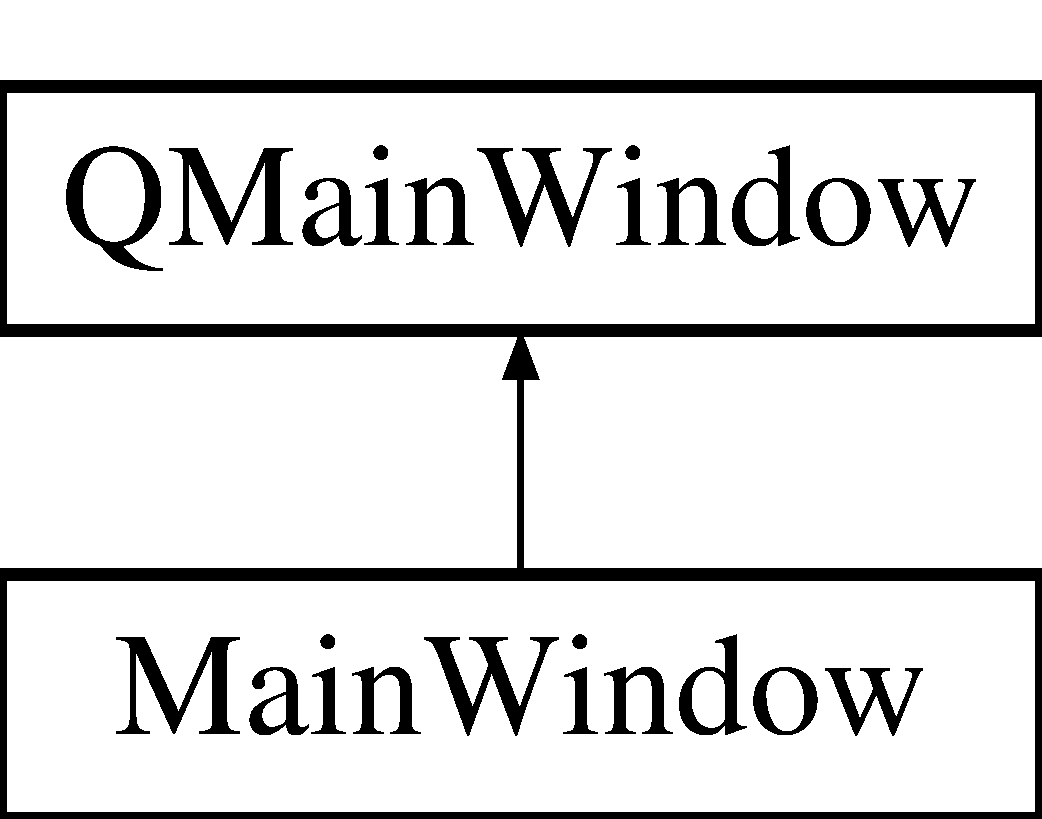
\includegraphics[height=2.000000cm]{class_main_window}
\end{center}
\end{figure}
\subsection*{Public Slots}
\begin{DoxyCompactItemize}
\item 
void \hyperlink{class_main_window_a0416fa37103aeb873f99c3c90f401f6f}{start\+\_\+level1} ()\hypertarget{class_main_window_a0416fa37103aeb873f99c3c90f401f6f}{}\label{class_main_window_a0416fa37103aeb873f99c3c90f401f6f}

\begin{DoxyCompactList}\small\item\em Create \hyperlink{classlevel1}{level1} and set it as the main widget. \end{DoxyCompactList}\item 
void \hyperlink{class_main_window_abba367075f5c8e11fdc9e531c55ef4e3}{start\+\_\+level2} ()\hypertarget{class_main_window_abba367075f5c8e11fdc9e531c55ef4e3}{}\label{class_main_window_abba367075f5c8e11fdc9e531c55ef4e3}

\begin{DoxyCompactList}\small\item\em Create \hyperlink{classlevel2}{level2} and set it as the main widget. \end{DoxyCompactList}\item 
void \hyperlink{class_main_window_a0be57e220676b7ff32fee2b9bd4dd8e8}{start\+\_\+level3} ()\hypertarget{class_main_window_a0be57e220676b7ff32fee2b9bd4dd8e8}{}\label{class_main_window_a0be57e220676b7ff32fee2b9bd4dd8e8}

\begin{DoxyCompactList}\small\item\em Create \hyperlink{classlevel3}{level3} and set it as the main widget. \end{DoxyCompactList}\item 
void \hyperlink{class_main_window_a982e9b59ebe751fe6b1aac349309a51f}{victory\+\_\+screen} ()\hypertarget{class_main_window_a982e9b59ebe751fe6b1aac349309a51f}{}\label{class_main_window_a982e9b59ebe751fe6b1aac349309a51f}

\begin{DoxyCompactList}\small\item\em Create the victory screen and set it as the main widget. \end{DoxyCompactList}\item 
void \hyperlink{class_main_window_ad095804e948ea80ebaa1311858700ded}{game\+\_\+over} ()\hypertarget{class_main_window_ad095804e948ea80ebaa1311858700ded}{}\label{class_main_window_ad095804e948ea80ebaa1311858700ded}

\begin{DoxyCompactList}\small\item\em Create the main menu screen and set it as the main widget. \end{DoxyCompactList}\item 
void \hyperlink{class_main_window_a565aac1b17c3810913270d503d94b983}{show\+\_\+controls} ()\hypertarget{class_main_window_a565aac1b17c3810913270d503d94b983}{}\label{class_main_window_a565aac1b17c3810913270d503d94b983}

\begin{DoxyCompactList}\small\item\em Create the game controls screen and set it as the main widget. \end{DoxyCompactList}\end{DoxyCompactItemize}
\subsection*{Public Member Functions}
\begin{DoxyCompactItemize}
\item 
\hyperlink{class_main_window_a8b244be8b7b7db1b08de2a2acb9409db}{Main\+Window} (Q\+Widget $\ast$parent=0)
\item 
\hyperlink{class_main_window_ae98d00a93bc118200eeef9f9bba1dba7}{$\sim$\+Main\+Window} ()\hypertarget{class_main_window_ae98d00a93bc118200eeef9f9bba1dba7}{}\label{class_main_window_ae98d00a93bc118200eeef9f9bba1dba7}

\begin{DoxyCompactList}\small\item\em Delete the main window. \end{DoxyCompactList}\end{DoxyCompactItemize}


\subsection{Detailed Description}
This class handles the UI displaying the main menu of the game. 

Definition at line 23 of file mainwindow.\+h.



\subsection{Constructor \& Destructor Documentation}
\index{Main\+Window@{Main\+Window}!Main\+Window@{Main\+Window}}
\index{Main\+Window@{Main\+Window}!Main\+Window@{Main\+Window}}
\subsubsection[{\texorpdfstring{Main\+Window(\+Q\+Widget $\ast$parent=0)}{MainWindow(QWidget *parent=0)}}]{\setlength{\rightskip}{0pt plus 5cm}Main\+Window\+::\+Main\+Window (
\begin{DoxyParamCaption}
\item[{Q\+Widget $\ast$}]{parent = {\ttfamily 0}}
\end{DoxyParamCaption}
)\hspace{0.3cm}{\ttfamily [explicit]}}\hypertarget{class_main_window_a8b244be8b7b7db1b08de2a2acb9409db}{}\label{class_main_window_a8b244be8b7b7db1b08de2a2acb9409db}
Create the main menu 
\begin{DoxyParams}{Parameters}
{\em parent} & is the parent Q\+Widget of this object \\
\hline
\end{DoxyParams}


Definition at line 10 of file mainwindow.\+cpp.


\begin{DoxyCode}
10                                       :
11     QMainWindow(parent),
12     ui(\textcolor{keyword}{new} Ui::MainWindow) \{
13     ui->setupUi(\textcolor{keyword}{this});
14     \textcolor{comment}{// Set up the music for the game}
15     menu\_music = \textcolor{keyword}{new} QMediaPlayer();
16     menu\_music->setMedia(QUrl(\textcolor{stringliteral}{"qrc:/sounds/menu.mp3"}));
17     menu\_music->play();
18     bgm = \textcolor{keyword}{new} QMediaPlayer();
19     bgm->setMedia(QUrl(\textcolor{stringliteral}{"qrc:/sounds/bgm.mp3"}));
20     victory\_music = \textcolor{keyword}{new} QMediaPlayer();
21     victory\_music->setMedia(QUrl(\textcolor{stringliteral}{"qrc:/sounds/victory.mp3"}));
22 \}
\end{DoxyCode}


The documentation for this class was generated from the following files\+:\begin{DoxyCompactItemize}
\item 
\hyperlink{mainwindow_8h}{mainwindow.\+h}\item 
\hyperlink{mainwindow_8cpp}{mainwindow.\+cpp}\end{DoxyCompactItemize}

\hypertarget{classvictory}{}\section{victory Class Reference}
\label{classvictory}\index{victory@{victory}}


This class handles the UI displaying the victory screen of the game.  




{\ttfamily \#include $<$victory.\+h$>$}

Inheritance diagram for victory\+:\begin{figure}[H]
\begin{center}
\leavevmode
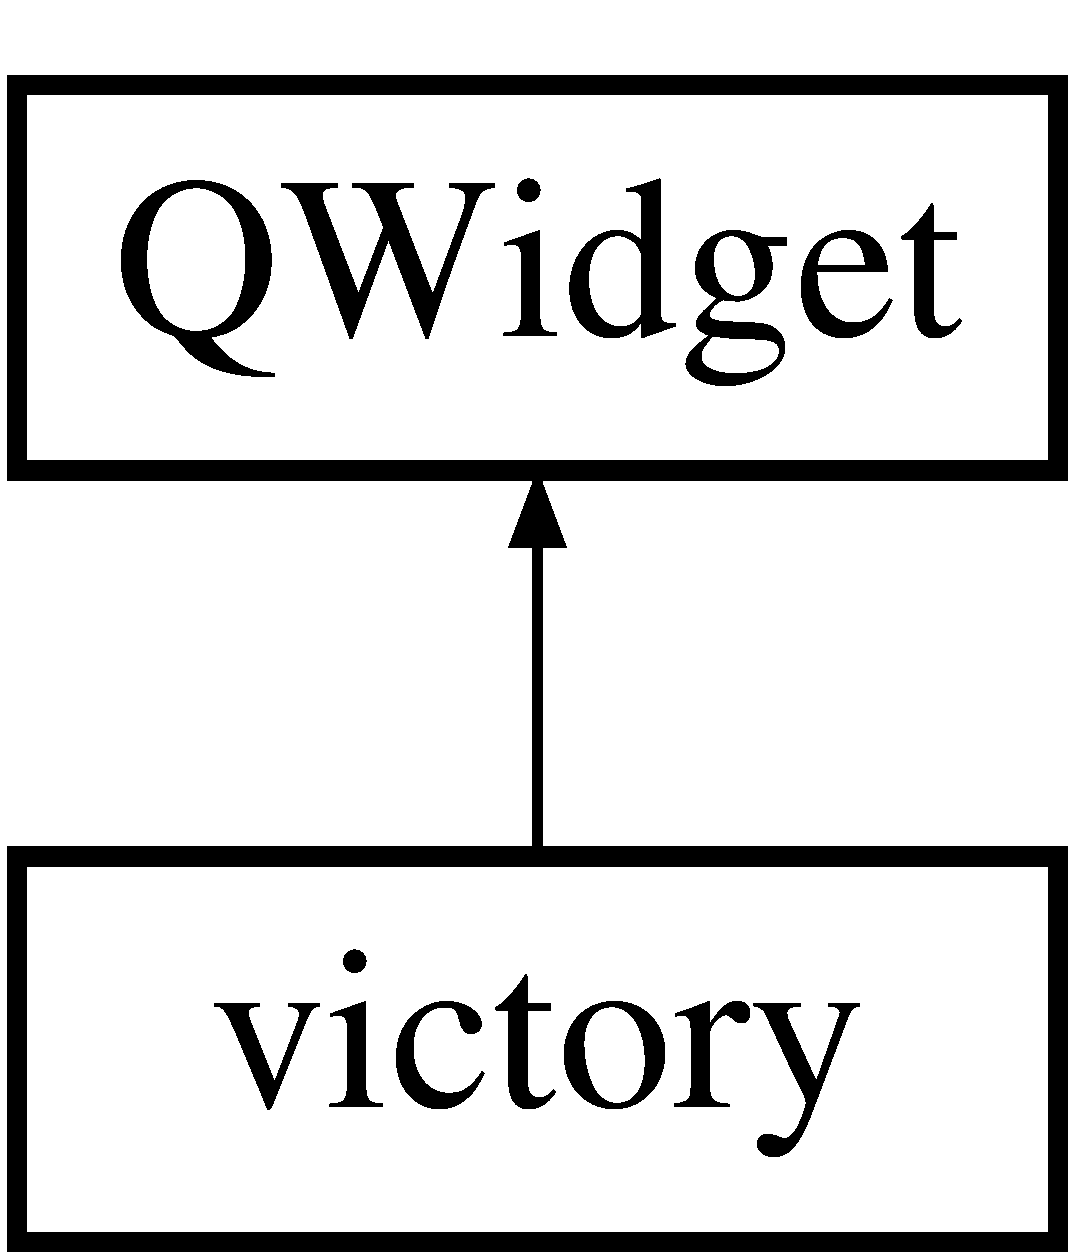
\includegraphics[height=2.000000cm]{classvictory}
\end{center}
\end{figure}
\subsection*{Public Member Functions}
\begin{DoxyCompactItemize}
\item 
\hyperlink{classvictory_a7d68234bd5e40dc9879caca6c2cdd4b3}{victory} (Q\+Widget $\ast$parent=0)
\item 
\hyperlink{classvictory_a6384ce7d94b46b7d07e8d870f939a863}{$\sim$victory} ()\hypertarget{classvictory_a6384ce7d94b46b7d07e8d870f939a863}{}\label{classvictory_a6384ce7d94b46b7d07e8d870f939a863}

\begin{DoxyCompactList}\small\item\em Delete the victory screen. \end{DoxyCompactList}\item 
void {\bfseries paint\+Event} (Q\+Paint\+Event $\ast$)\hypertarget{classvictory_a95c8578693a125725cf4d64694436eed}{}\label{classvictory_a95c8578693a125725cf4d64694436eed}

\end{DoxyCompactItemize}


\subsection{Detailed Description}
This class handles the UI displaying the victory screen of the game. 

Definition at line 20 of file victory.\+h.



\subsection{Constructor \& Destructor Documentation}
\index{victory@{victory}!victory@{victory}}
\index{victory@{victory}!victory@{victory}}
\subsubsection[{\texorpdfstring{victory(\+Q\+Widget $\ast$parent=0)}{victory(QWidget *parent=0)}}]{\setlength{\rightskip}{0pt plus 5cm}victory\+::victory (
\begin{DoxyParamCaption}
\item[{Q\+Widget $\ast$}]{parent = {\ttfamily 0}}
\end{DoxyParamCaption}
)\hspace{0.3cm}{\ttfamily [explicit]}}\hypertarget{classvictory_a7d68234bd5e40dc9879caca6c2cdd4b3}{}\label{classvictory_a7d68234bd5e40dc9879caca6c2cdd4b3}
Create the victory screen 
\begin{DoxyParams}{Parameters}
{\em parent} & is the parent Q\+Widget of this object \\
\hline
\end{DoxyParams}


Definition at line 10 of file victory.\+cpp.


\begin{DoxyCode}
10                                 : QWidget(parent), ui(\textcolor{keyword}{new} Ui::victory)\{
11     \textcolor{comment}{// init ui form's components}
12     ui->setupUi(\textcolor{keyword}{this});
13     connect(ui->pushButton, SIGNAL(clicked(\textcolor{keywordtype}{bool})), parent, SLOT(game\_over()));
14 \}
\end{DoxyCode}


The documentation for this class was generated from the following files\+:\begin{DoxyCompactItemize}
\item 
\hyperlink{victory_8h}{victory.\+h}\item 
\hyperlink{victory_8cpp}{victory.\+cpp}\end{DoxyCompactItemize}

\chapter{File Documentation}
\hypertarget{controls_8cpp}{}\section{controls.\+cpp File Reference}
\label{controls_8cpp}\index{controls.\+cpp@{controls.\+cpp}}
{\ttfamily \#include \char`\"{}controls.\+h\char`\"{}}\\*


\subsection{Detailed Description}
\begin{DoxyAuthor}{Author}
Matthew Chan 
\end{DoxyAuthor}
\begin{DoxyDate}{Date}
March 9, 2016 
\end{DoxyDate}

\hypertarget{controls_8h}{}\section{controls.\+h File Reference}
\label{controls_8h}\index{controls.\+h@{controls.\+h}}
{\ttfamily \#include $<$Q\+Main\+Window$>$}\\*
{\ttfamily \#include \char`\"{}ui\+\_\+controls.\+h\char`\"{}}\\*
{\ttfamily \#include $<$Q\+Painter$>$}\\*
\subsection*{Classes}
\begin{DoxyCompactItemize}
\item 
class \hyperlink{classcontrols}{controls}
\begin{DoxyCompactList}\small\item\em This class handles the UI displaying the controls/instructions for the game. \end{DoxyCompactList}\end{DoxyCompactItemize}


\subsection{Detailed Description}
\begin{DoxyAuthor}{Author}
Matthew Chan 
\end{DoxyAuthor}
\begin{DoxyDate}{Date}
March 9, 2016 
\end{DoxyDate}

\hypertarget{level1_8cpp}{}\section{level1.\+cpp File Reference}
\label{level1_8cpp}\index{level1.\+cpp@{level1.\+cpp}}
{\ttfamily \#include \char`\"{}level1.\+h\char`\"{}}\\*


\subsection{Detailed Description}
\begin{DoxyAuthor}{Author}
Matthew Chan 
\end{DoxyAuthor}
\begin{DoxyDate}{Date}
March 9, 2016 
\end{DoxyDate}

\hypertarget{level1_8h}{}\section{level1.\+h File Reference}
\label{level1_8h}\index{level1.\+h@{level1.\+h}}
{\ttfamily \#include $<$Q\+Main\+Window$>$}\\*
{\ttfamily \#include \char`\"{}ui\+\_\+level1.\+h\char`\"{}}\\*
{\ttfamily \#include \char`\"{}ui\+\_\+mainwindow.\+h\char`\"{}}\\*
{\ttfamily \#include $<$Q\+Painter$>$}\\*
{\ttfamily \#include $<$Q\+Pixmap$>$}\\*
{\ttfamily \#include $<$Q\+Timer$>$}\\*
{\ttfamily \#include $<$Q\+Point$>$}\\*
{\ttfamily \#include $<$Q\+Size$>$}\\*
{\ttfamily \#include $<$Q\+Key\+Event$>$}\\*
{\ttfamily \#include $<$Q\+Media\+Player$>$}\\*
\subsection*{Classes}
\begin{DoxyCompactItemize}
\item 
class \hyperlink{classlevel1}{level1}
\begin{DoxyCompactList}\small\item\em This class handles the logic and display events for level 1. \end{DoxyCompactList}\end{DoxyCompactItemize}


\subsection{Detailed Description}
\begin{DoxyAuthor}{Author}
Matthew Chan 
\end{DoxyAuthor}
\begin{DoxyDate}{Date}
March 9, 2016 
\end{DoxyDate}

\hypertarget{level2_8cpp}{}\section{level2.\+cpp File Reference}
\label{level2_8cpp}\index{level2.\+cpp@{level2.\+cpp}}
{\ttfamily \#include \char`\"{}level2.\+h\char`\"{}}\\*


\subsection{Detailed Description}
\begin{DoxyAuthor}{Author}
Matthew Chan 
\end{DoxyAuthor}
\begin{DoxyDate}{Date}
March 9, 2016 
\end{DoxyDate}

\hypertarget{level2_8h}{}\section{level2.\+h File Reference}
\label{level2_8h}\index{level2.\+h@{level2.\+h}}
{\ttfamily \#include $<$Q\+Main\+Window$>$}\\*
{\ttfamily \#include \char`\"{}ui\+\_\+level2.\+h\char`\"{}}\\*
{\ttfamily \#include \char`\"{}ui\+\_\+mainwindow.\+h\char`\"{}}\\*
{\ttfamily \#include $<$Q\+Painter$>$}\\*
{\ttfamily \#include $<$Q\+Pixmap$>$}\\*
{\ttfamily \#include $<$Q\+Timer$>$}\\*
{\ttfamily \#include $<$Q\+Point$>$}\\*
{\ttfamily \#include $<$Q\+Size$>$}\\*
{\ttfamily \#include $<$Q\+Key\+Event$>$}\\*
{\ttfamily \#include $<$chrono$>$}\\*
{\ttfamily \#include $<$random$>$}\\*
{\ttfamily \#include $<$Q\+Media\+Player$>$}\\*
\subsection*{Classes}
\begin{DoxyCompactItemize}
\item 
class \hyperlink{classlevel2}{level2}
\begin{DoxyCompactList}\small\item\em This class handles the logic and display events for level 2. \end{DoxyCompactList}\end{DoxyCompactItemize}


\subsection{Detailed Description}
\begin{DoxyAuthor}{Author}
Matthew Chan 
\end{DoxyAuthor}
\begin{DoxyDate}{Date}
March 9, 2016 
\end{DoxyDate}

\hypertarget{level3_8cpp}{}\section{level3.\+cpp File Reference}
\label{level3_8cpp}\index{level3.\+cpp@{level3.\+cpp}}
{\ttfamily \#include \char`\"{}level3.\+h\char`\"{}}\\*


\subsection{Detailed Description}
\begin{DoxyAuthor}{Author}
Matthew Chan 
\end{DoxyAuthor}
\begin{DoxyDate}{Date}
March 9, 2016 
\end{DoxyDate}

\hypertarget{level3_8h}{}\section{level3.\+h File Reference}
\label{level3_8h}\index{level3.\+h@{level3.\+h}}
{\ttfamily \#include $<$Q\+Main\+Window$>$}\\*
{\ttfamily \#include \char`\"{}ui\+\_\+level3.\+h\char`\"{}}\\*
{\ttfamily \#include \char`\"{}ui\+\_\+mainwindow.\+h\char`\"{}}\\*
{\ttfamily \#include $<$Q\+Painter$>$}\\*
{\ttfamily \#include $<$Q\+Pixmap$>$}\\*
{\ttfamily \#include $<$Q\+Timer$>$}\\*
{\ttfamily \#include $<$Q\+Point$>$}\\*
{\ttfamily \#include $<$Q\+Size$>$}\\*
{\ttfamily \#include $<$Q\+Key\+Event$>$}\\*
{\ttfamily \#include $<$Q\+Media\+Player$>$}\\*
\subsection*{Classes}
\begin{DoxyCompactItemize}
\item 
class \hyperlink{classlevel3}{level3}
\begin{DoxyCompactList}\small\item\em This class handles the logic and display events for level 3. \end{DoxyCompactList}\end{DoxyCompactItemize}


\subsection{Detailed Description}
\begin{DoxyAuthor}{Author}
Matthew Chan 
\end{DoxyAuthor}
\begin{DoxyDate}{Date}
March 9, 2016 
\end{DoxyDate}

\hypertarget{main_8cpp}{}\section{main.\+cpp File Reference}
\label{main_8cpp}\index{main.\+cpp@{main.\+cpp}}


This is the main() function for the Space Invaders game.  


{\ttfamily \#include \char`\"{}mainwindow.\+h\char`\"{}}\\*
{\ttfamily \#include $<$Q\+Application$>$}\\*
\subsection*{Functions}
\begin{DoxyCompactItemize}
\item 
int {\bfseries main} (int argc, char $\ast$argv\mbox{[}$\,$\mbox{]})\hypertarget{main_8cpp_a0ddf1224851353fc92bfbff6f499fa97}{}\label{main_8cpp_a0ddf1224851353fc92bfbff6f499fa97}

\end{DoxyCompactItemize}


\subsection{Detailed Description}
This is the main() function for the Space Invaders game. 

\begin{DoxyAuthor}{Author}
Matthew Chan 
\end{DoxyAuthor}
\begin{DoxyDate}{Date}
March 9, 2016 
\end{DoxyDate}

\hypertarget{mainwindow_8cpp}{}\section{mainwindow.\+cpp File Reference}
\label{mainwindow_8cpp}\index{mainwindow.\+cpp@{mainwindow.\+cpp}}
{\ttfamily \#include \char`\"{}mainwindow.\+h\char`\"{}}\\*
{\ttfamily \#include \char`\"{}ui\+\_\+mainwindow.\+h\char`\"{}}\\*


\subsection{Detailed Description}
\begin{DoxyAuthor}{Author}
Matthew Chan 
\end{DoxyAuthor}
\begin{DoxyDate}{Date}
March 9, 2016 
\end{DoxyDate}

\hypertarget{mainwindow_8h}{}\section{mainwindow.\+h File Reference}
\label{mainwindow_8h}\index{mainwindow.\+h@{mainwindow.\+h}}
{\ttfamily \#include $<$Q\+Main\+Window$>$}\\*
{\ttfamily \#include $<$Q\+Media\+Player$>$}\\*
{\ttfamily \#include \char`\"{}victory.\+h\char`\"{}}\\*
{\ttfamily \#include \char`\"{}level1.\+h\char`\"{}}\\*
{\ttfamily \#include \char`\"{}level2.\+h\char`\"{}}\\*
{\ttfamily \#include \char`\"{}level3.\+h\char`\"{}}\\*
{\ttfamily \#include \char`\"{}controls.\+h\char`\"{}}\\*
\subsection*{Classes}
\begin{DoxyCompactItemize}
\item 
class \hyperlink{class_main_window}{Main\+Window}
\begin{DoxyCompactList}\small\item\em This class handles the UI displaying the main menu of the game. \end{DoxyCompactList}\end{DoxyCompactItemize}


\subsection{Detailed Description}
\begin{DoxyAuthor}{Author}
Matthew Chan 
\end{DoxyAuthor}
\begin{DoxyDate}{Date}
March 9, 2016 
\end{DoxyDate}

\hypertarget{victory_8cpp}{}\section{victory.\+cpp File Reference}
\label{victory_8cpp}\index{victory.\+cpp@{victory.\+cpp}}
{\ttfamily \#include \char`\"{}victory.\+h\char`\"{}}\\*


\subsection{Detailed Description}
\begin{DoxyAuthor}{Author}
Matthew Chan 
\end{DoxyAuthor}
\begin{DoxyDate}{Date}
March 9, 2016 
\end{DoxyDate}

\hypertarget{victory_8h}{}\section{victory.\+h File Reference}
\label{victory_8h}\index{victory.\+h@{victory.\+h}}
{\ttfamily \#include $<$Q\+Main\+Window$>$}\\*
{\ttfamily \#include \char`\"{}ui\+\_\+victory.\+h\char`\"{}}\\*
{\ttfamily \#include $<$Q\+Painter$>$}\\*
\subsection*{Classes}
\begin{DoxyCompactItemize}
\item 
class \hyperlink{classvictory}{victory}
\begin{DoxyCompactList}\small\item\em This class handles the UI displaying the victory screen of the game. \end{DoxyCompactList}\end{DoxyCompactItemize}


\subsection{Detailed Description}
\begin{DoxyAuthor}{Author}
Matthew Chan 
\end{DoxyAuthor}
\begin{DoxyDate}{Date}
March 9, 2016 
\end{DoxyDate}

%--- End generated contents ---

% Index
\backmatter
\newpage
\phantomsection
\clearemptydoublepage
\addcontentsline{toc}{chapter}{Index}
\printindex

\end{document}
